\documentclass[preprint,12pt,authoryear]{elsarticle}
\usepackage{amsmath,amssymb,amsthm}
\usepackage{booktabs}
\usepackage{graphicx}
\usepackage{xcolor}
\usepackage{adjustbox}
\usepackage{hyperref}
\usepackage{algorithm}
\usepackage{algpseudocode}
\newtheorem{proposition}{Proposition}
\newtheorem{assumption}{Assumption}
\newcommand{\E}{\mathbb{E}}
\newcommand{\qp}{QP-LightGCN}
\newcommand{\Yhat}{\hat Y}
\begin{document}
\begin{frontmatter}
\title{What carries the gains of debiased graph recommendation? A controlled study on four benchmarks with unbiased test data}
\author{Anonymous}
\begin{abstract}
Under one controlled protocol, the gains reported for graph exposure-bias corrections depend strongly on evaluation choices, and third-party corrections add little over an equally tuned backbone. We re-evaluate these corrections on Coat, Yahoo! R3, KuaiRand-Pure and KuaiRec. Uniform data serve only for validation and testing, except Coat's shipped propensities, which are checked for the prior rows only. Configurations are selected per split on validation data, and leading methods are retrained with three seeds. Four findings follow. Selecting on test data inflates Coat scores by up to $0.030$ nDCG@5. Third-party debiasers improve LightGCN by point-estimate gains of at most $4.10\times10^{-3}$ nDCG on Coat, Yahoo! R3 and KuaiRand-Pure, and none survives a correction for overlapping splits there. An additive prior fitted on the exposed log gives the largest point-estimate gains over LightGCN, $31.98\times10^{-3}$ on Coat and $21.22\times10^{-3}$ on KuaiRec. The Coat gain is not robust to that correction, the KuaiRec gain is, and the mechanism is not identified. Making the multi-hop propagation exactly unbiased does not improve ranking on the three real logs where it was run. The scope is four public benchmarks, offline evaluation and implicit-feedback learners. We propose no new estimator.

\end{abstract}
\begin{keyword}
recommender systems \sep exposure bias \sep graph collaborative filtering \sep propensity \sep doubly robust
\end{keyword}
\end{frontmatter}
\section{Introduction}\label{sec:intro}

Under one controlled protocol with unbiased test data, the gains reported for exposure-bias corrections of graph
recommenders depend strongly on evaluation choices, and third-party corrections add little over an equally tuned
backbone.

Graph-based recommenders represent users and items as nodes and score a user-item pair by propagating embeddings over
the user-item graph. LightGCN \citep{he2020lightgcn} is a standard backbone of this family, and it is usually trained on
implicit feedback logs. In such a log an interaction is recorded only when the item was shown and the user responded.
The logged graph therefore reflects the exposure policy as well as user taste \citep{marlin2009collaborative,chen2023bias},
and a model fitted to the log treats every absence as informative. The pairwise loss that trains LightGCN, Bayesian
personalised ranking \citep{rendle2009bpr}, draws its negatives uniformly from the items the user has no logged
interaction with. Under exposure bias most of these items were never shown. Corrections act on the loss
\citep{schnabel2016,wang2019drjl,guo2021mrdr}, on the latent exposure or on the likelihood weights
\citep{liang2016exposure,saito2020unbiased}, and, for graph models, on aggregation or adjacency
\citep{kim2022navip,zhao2022radjnorm,islam2026ppd}.

This paper starts from the two nuisance functions that a DR estimator already fits: an exposure propensity $p_{ui}$ and
an imputed preference $\Yhat_{ui}$. Under an independence assumption between exposure and preference given covariates,
Bayes' rule gives the probability that a pair absent from the log is a positive,
\begin{equation}\label{eq:Qintro}
Q_{ui}=\Pr\bigl(Y_{ui}=1\mid O_{ui}Y_{ui}=0,\,x_{ui}\bigr)
=\frac{\Yhat_{ui}\,(1-p_{ui})}{1-p_{ui}\,\Yhat_{ui}}.
\end{equation}
The candidate models use $Q$ in two places inside an otherwise unchanged LightGCN. Each sampled BPR negative is
down-weighted by $1-Q_{uj}$, and the standardised logit of the imputation is added to the score as a fixed offset whose
weight is chosen on validation data. Both nuisance functions are fitted on the biased log before training. The one
exception to the rule that training uses no uniformly collected data is Coat, whose shipped propensities were estimated
by the dataset authors from a uniform sample. We call the full model QP-LightGCN and evaluate it with its variants as one
family.

The gains reported for these corrections are hard to compare, for three reasons. First, the studies use uniformly
collected data in different ways: some train on it, some select configurations on it, and some use it only for testing
(Section~\ref{sec:related}). Second, tuning budgets differ, so a method given a larger search space can obtain a higher
test score through selection alone. Third, single runs are common, and the ordering of close methods can depend on the
random seed. Our own runs illustrate the third point. In the main run, QP-LightGCN is above iALS on Coat by
$+20.02\times10^{-3}$ [19.74], which is nominally significant after Holm correction over the eight baseline comparisons
($p_\mathrm{Holm}=0.047$). When the selected configurations are retrained with seeds 1 to 3, the difference is
$+3.39\times10^{-3}$ [20.70], with $p_\mathrm{Holm}=0.75$ over the two baseline comparisons of that check. These seed
comparisons are descriptive, because the two baselines of each dataset were chosen on test data.

The study asks four research questions, which Table~\ref{tab:rq} answers and locates.

\begin{table}[htbp]\centering\footnotesize
\caption{Research questions, short answers and the sections that answer them.}\label{tab:rq}
\begin{tabular}{p{4.6cm}p{7.2cm}l}
\toprule
Question & Short answer & Section \\
\midrule
RQ1: How much do evaluation choices change the conclusions? & A lot. Selection on the test split inflates scores and can reverse an order. Many pairwise signs depend on the search budget, the seed or the metric. & Section~\ref{sec:res-eval} \\
RQ2: How much do graph-specific corrections add over an equally tuned backbone? & Little, on Coat, Yahoo! R3 and KuaiRand-Pure. On KuaiRec the gains are larger, and a pointwise loss without debiasing gives a larger difference of means. & Section~\ref{sec:res-debias} \\
RQ3: Which ingredient carries the gains that remain? & An additive prior fitted once on the exposed log. Its inverse-propensity weights are not what matters in our runs, and the mechanism is not identified. & Section~\ref{sec:res-ingredient} \\
RQ4: Does exact unbiasedness of the propagation matter for ranking? & Not on the three real logs on which it was run. & Section~\ref{sec:res-walk} \\
\bottomrule
\end{tabular}
\end{table}

The paper makes four contributions. None of them is a new estimator.
\begin{enumerate}
\item \emph{Protocol and its sensitivity (RQ1).} Four public benchmarks with unbiased test data, uniform data used only for
validation and testing, per-split selection on validation data, per-user paired tests with Holm correction, and
retraining with seeds. Selecting on the test split inflates Coat scores by up to $0.030$ nDCG@5.
\item \emph{Third-party debiasers add little over an equally tuned backbone (RQ2).} On Coat, Yahoo! R3 and KuaiRand-Pure
the largest point-estimate gain of a third-party debiaser over LightGCN is $+4.10\times10^{-3}$ nDCG, and none of these
gains survives a correction for overlapping splits on those datasets.
\item \emph{Prior anatomy (RQ3).} The gains over the backbone that the additive prior provides are examined with controls.
Removing its inverse-propensity weights does not reduce them, a shuffled item term removes the KuaiRec gain, and
popularity does not reproduce it. The mechanism is not identified.
\item \emph{A negative result on walk correction (RQ4).} The walk correction of DRUP removes the repeated-edge bias of
multi-hop DR propagation. It does not improve ranking on Coat, Yahoo! R3 or KuaiRec.
\end{enumerate}

The QP-LightGCN family and its refinements are members of the evaluated family (\ref{app:refine}), not
contributions in their own right. We do not claim that debiasing is useless in general.

The scope is four public benchmarks, offline evaluation, top-$K$ nDCG at the cut-off used for each dataset (5 for Coat
and Yahoo! R3, 10 for KuaiRand-Pure, 20 for KuaiRec), and implicit-feedback learners trained on the biased log. The
walk-correction claim concerns Coat, Yahoo! R3 and KuaiRec, the three real logs on which DR and DRUP were run. Coat has
225 evaluated users, so its power is low. For Coat we report the differences that the data exclude, and we do not report
equality. We do not claim that AdvInfoNCE, NAVIP, r-AdjNorm, SimGCL or MACR fail in general. Our implementations, tuned
with the stated budgets under this protocol, do not beat the backbone by more than the amounts reported. We do not give a
mechanism for why the prior helps beyond the controls of Section~\ref{sec:res-ingredient}, and the reading that the
prior acts as a debiased item-quality score is a hypothesis.

\section{Related work}\label{sec:related}

\subsection{Graph collaborative filtering and graph debiasing}\label{sec:related-graph}

LightGCN \citep{he2020lightgcn} is the backbone used in our experiments. Other graph
convolutional recommenders include NGCF \citep{wang2019ngcf} and UltraGCN
\citep{mao2021ultragcn}, and contrastive graph variants include SGL \citep{wu2021sgl} and
SimGCL \citep{yu2022simgcl}. Linear and closed-form models include EASE \citep{steck2019ease},
GF-CF \citep{shen2021gfcf} and BSPM \citep{choi2023bspm}. Weighted matrix factorisation for
implicit feedback, iALS \citep{hu2008ials}, is a standard baseline, and \citet{rendle2022ials}
revisit its tuning on item recommendation benchmarks. \citet{wu2022gnnsurvey} survey graph
neural recommenders. These models fit or propagate over the logged graph and do not model
which pairs were exposed.

Graph models have also been debiased. NAVIP \citep{kim2022navip} weights neighbour
aggregation by inverse propensities. r-AdjNorm \citep{zhao2022radjnorm} tunes the strength of
adjacency normalisation to trade accuracy against novelty, and \citet{chen2024gcnpop} study
how graph convolutions can amplify popularity bias. APDA \citep{zhou2023apda} and CAGED
\citep{que2025caged} learn aggregation weights, and DPAA \citep{dpaa2026}, an arXiv preprint,
re-weights message passing. AdvDrop \citep{zhang2024advdrop} learns an adversarial edge dropout
on the interaction graph and reports IPS and DR baselines on Coat, Yahoo! R3 and KuaiRec. PPD
\citep{islam2026ppd} removes a popularity direction from pre-trained LightGCN embeddings
without retraining, and is evaluated on KuaiRec, Coat and Yahoo! R3. DR-GNN
\citep{wang2024drgnn} applies distributionally robust optimisation over graph neighbourhoods;
its ``DR'' stands for distributionally robust, not doubly robust. The popularity-debiasing
methods MACR \citep{wei2021macr} and PDA \citep{zhang2021pda} are used as baselines in our
study. Most of these methods act on aggregation, adjacency, embeddings or a robust objective,
rather than on the negatives of the pairwise loss.

\subsection{Propensity, doubly robust and negative-weighting methods}\label{sec:related-dr}

Ratings and implicit feedback are missing not at random \citep{marlin2009collaborative}, and
surveys organise the resulting biases and the causal methods that address them
\citep{chen2023bias,gao2024causalsurvey}. Propensity methods re-weight the loss by inverse
propensities or self-normalised estimators \citep{schnabel2016,swaminathan2015snips,saito2020unbiased}.
\citet{steck2010mnar} showed that missing ratings carry information, proposed test measures
that can be estimated without bias when ratings are missing not at random, and derived training
objectives that account for the missing entries. Doubly robust learning adds an imputation model
to the inverse-propensity estimator \citep{wang2019drjl}, and later doubly robust variants
address related debiasing problems \citep{guo2021mrdr,dai2022gdr,li2023stabledr}. Information-theoretic counterfactual
learning from missing-not-at-random feedback is studied by \citet{wang2020cvib}.

Some debiasing methods use a small uniform sample for training. AutoDebias
\citep{chen2021autodebias} learns sample weights and an imputation function by bi-level
meta-learning on a small uniform sample. CausE \citep{bonner2018cause} embeds a small randomised
sample alongside the logged one, and KDCRec \citep{liu2020kdcrec} distils from a model fitted on
uniform data into a model trained on the biased log.

The methods closest to our negative weighting are those for exposure and false negatives. ExpoMF
\citep{liang2016exposure} infers an exposure posterior for unclicked items inside a matrix
factorisation model. Rel-MF \citep{saito2020unbiased} re-weights observations by propensity, and
unbiased pairwise learning \citep{saito2020ictir} applies the same idea to pairwise objectives.
SRNS \citep{ding2020srns} identifies likely false negatives during sampling, and debiased
contrastive learning \citep{chuang2020dcl} corrects negatives that are in fact positives. In
contrastive collaborative filtering, the BC loss \citep{zhang2022bc} adds a margin that depends
on the popularity-bias degree of each interaction, and AdvInfoNCE \citep{zhang2023advinfonce}
assigns each negative an adversarially learned hardness weight. Correct-and-Weight
\citep{yin2026cw}, an arXiv preprint, weights negatives against false negatives and is tested
with graph backbones on random splits. Exposure-aware negative sampling for graph recommenders
uses in-community popularity as a proxy for exposure \citep{chen2026icpns}, also an arXiv
preprint. The original formulations of ExpoMF, SRNS, debiased contrastive learning and
AdvInfoNCE do not combine a propensity with an imputation of the kind a doubly robust estimator
provides. IPS-weighted BPR on LightGCN has been studied with simulated propensities
\citep{raja2025ipsbpr}.

The offset used by our candidate models is a fixed, standardised imputation logit added to the
score. Adding a fixed offset is a familiar device. In long-tail classification, logit adjustment
adds a class prior to the logits \citep{menon2021logit}. The offset used here differs in one
respect: it is a debiased estimate of item-level preference, obtained from an
inverse-propensity-weighted imputation, and not a class prior.

\subsection{Evaluation and reproducibility}\label{sec:related-eval}

Several studies have shown that comparisons between recommenders depend on the protocol.
\citet{dacrema2019progress} re-ran recent neural recommenders against simple baselines and found
that several did not outperform well-tuned versions of those baselines. \citet{rendle2019baselines}
argue that baselines in published comparisons are often under-tuned, so that a reported gain
depends on the effort spent on each method. \citet{rendle2022ials} show that iALS, when tuned
carefully, is competitive on common item recommendation benchmarks. \citet{anelli2023myth}
question the reported advances of graph collaborative filtering.

Several parts of the protocol can change a conclusion. Sampled and exact metrics can disagree
\citep{krichene2020sampled}. \citet{nadeau2003} propose a corrected resampled t-test for the generalisation error, for
resamples that overlap. Reporting the expected
validation performance as a function of the number of configurations tried makes the tuning
budget visible \citep{dodge2019showyourwork}. Comparisons over several methods and datasets also
need a multiple-testing correction, for which we use the step-down procedure of
\citet{holm1979}.

\subsection{Gap and positioning}\label{sec:related-gap}

The contribution of this paper is evidence rather than a new method. The graph debiasers and the
candidate models of Section~\ref{sec:methods} are evaluated under one protocol, and the study measures how far
each conclusion depends on evaluation choices. Table~\ref{tab:positioning} summarises how the
related studies use uniformly collected data and which benchmarks they use. The uses differ.
Some studies train on uniform data (AutoDebias, CausE, ConAlign), some select configurations on
part of it (CDR, PPD, ConAlign), and some keep it out of both training and selection (DCE, BISER).

\begin{table}[t]
\centering
\caption{Positioning of related studies by their protocol. Entries follow the protocols as
described in the cited papers; ``not stated'' marks a point that the description does not
settle. Uniform data are the uniformly collected or randomised samples of the benchmark.}
\label{tab:positioning}
\footnotesize
\adjustbox{max width=\textwidth}{%
\begin{tabular}{p{2.6cm}p{1.9cm}p{2.5cm}p{2.0cm}p{2.6cm}p{2.4cm}}
\toprule
Study & Graph backbone & Propensity or imputation & Uniform data in training & Uniform data for validation or selection & Unbiased test benchmarks \\
\midrule
AutoDebias \citep{chen2021autodebias} & no (matrix factorisation) & learned weights and imputation & yes, small sample & yes, small sample & Coat, Yahoo! R3 \\
CausE \citep{bonner2018cause} & no (matrix factorisation) & none & yes, randomised sample & no, validation from logged policy & MovieLens, Netflix \\
CDR \citep{song2023cdr} & no (matrix factorisation) & doubly robust family & no & yes, part of unbiased data & Coat, Yahoo! R3, KuaiRand \\
DCE \citep{kweon2024dce} & no (MF or NCF) & doubly robust loss & no & no, held out from biased training data & Coat, Yahoo! R3, KuaiRec \\
BISER \citep{lee2022biser} & no & self-inverse propensity & no & no, held out from biased training data & Coat, Yahoo! R3 \\
ConAlign \citep{zhang2026conalign} & no (dual tower) & MF-IPS and MF-DR baselines & yes & yes & Coat, Yahoo! R3, KuaiRand-Pure \\
NAVIP \citep{kim2022navip} & yes & inverse propensity on edges & no & pseudo-unbiased popularity sample & Yahoo! R3 and pseudo-unbiased sets \\
AdvDrop \citep{zhang2024advdrop} & yes & IPS and DR baselines only & no, for its own method & not stated & Coat, Yahoo!, KuaiRec \\
PPD \citep{islam2026ppd} & yes, post hoc & none & no & yes on Coat and KuaiRec; biased sample on Yahoo! R3 & Coat, Yahoo! R3, KuaiRec \\
DPAA \citep{dpaa2026} & yes & none & no & validation present, construction not confirmed & Coat, Yahoo! R3, KuaiRec \\
DR-GNN \citep{wang2024drgnn} & yes & none & not stated & not stated & Coat, Yahoo \\
\midrule
This study & yes & IPS-fitted imputation and propensity & no, except Coat shipped propensities & yes & Coat, Yahoo! R3, KuaiRand-Pure, KuaiRec \\
\bottomrule
\end{tabular}}
\end{table}

A web search in October 2026 found no graph recommender that uses a posterior probability,
built from a propensity and an imputation, to weight sampled negatives, and none that adds a
debiased imputation to a graph model's score. It also found no graph study that uses
KuaiRand-Pure. The search used general web sources and cannot be exhaustive. Coat, Yahoo! R3 and
KuaiRec are already used for graph debiasing by AdvDrop, PPD and DPAA. We therefore do not claim
that the posterior weighting or the imputation offset is new. The claim we make is narrower: we
found no study that evaluates graph debiasers on all four benchmarks under one protocol, with
uniform data excluded from training, and with an analysis of how the budget and the selection
rule change the conclusions.

%======================================================================
\section{Protocol}\label{sec:protocol}
%======================================================================

The protocol rests on one rule. Uniformly collected data are read only to choose among trained models
and to measure them. They never enter a training objective, a nuisance model that a trained model uses,
or the stopping of training. This section states the controls that enforce the rule, how the splits,
the selection and the seeds are built, how the tests and sensitivity margins are defined, and how the
stored results were reconciled before the analysis. The methods to which the protocol is applied are
listed in Section~\ref{sec:methods}.

\subsection{Where each data source may enter}\label{sec:leakage}

Table~\ref{tab:leakage} lists the stages of the pipeline and the data each stage may read. ``Log'' is the
biased training log, which holds the exposure matrix and the outcomes of the exposed pairs.
``Validation'' and ``test'' are the parts of the uniformly collected data that a split assigns to each role.

\begin{table}[htbp]\centering\footnotesize
\caption{Permitted uses of each data source. The Coat row for the propensity is the one exception to the
rule, and it is discussed in the text.}\label{tab:leakage}
\begin{tabular}{lccc}
\toprule
Stage & Log & Validation & Test \\
\midrule
Exposure propensity $\hat p$ (Coat: shipped, see text) & yes & no & no \\
Additive imputation $\hat Y$, prior $z$, weights $Q$ & yes & no & no \\
Cross-fitted nuisances of the DRGP prior & yes & no & no \\
Training of every model & yes & no & no \\
Choice of configuration and epoch within a split & no & yes & no \\
Early stopping within a split & no & yes & no \\
Reported test score of the chosen model & no & no & yes \\
\bottomrule
\end{tabular}
\end{table}

The additive imputation is fitted on the log without cross-fitting, so the same log supplies $\hat Y$ and the
training data. The DRGP prior of \ref{sec:drgp} is cross-fitted over ten folds before its
coefficients are fitted. Test scores are computed after every epoch and stored, but no choice reads them.
The sensitivity analysis of the results reads them only to measure what selection on test data would
change, and it does not report such a selection as a method.

\paragraph{The Coat exception.}
The shipped Coat propensities were estimated by the dataset authors from a uniformly collected
sample~\citep{schnabel2016}. That sample is also the source of our validation and test data, so uniform
data reach a training input on Coat, indirectly. Every propensity-based row on Coat uses these
propensities: DR-LightGCN, NAVIP, DR-JL, MRDR, DR adjacency, DRUP and the prior rows. To check the effect
on the prior rows, we refitted them with propensities estimated from the log by the logistic model of
Section~\ref{sec:prior}. Table~\ref{tab:T10} gives the results. Relative to their no-prior backbones, the
prior gains are $+19.44\times10^{-3}$ [18.66] for iALS-p and $+33.62\times10^{-3}$ [16.72] for LightGCN-p
with estimated propensities. With the shipped propensities they are $+16.82\times10^{-3}$ [18.04] and
$+31.98\times10^{-3}$ [20.65]. The paired differences between the two propensity inputs are
$+2.63\times10^{-3}$ [5.27] for iALS-p and $+1.64\times10^{-3}$ [10.30] for LightGCN-p, with
$p_\mathrm{Holm}=1.000$ in both cases. The values in brackets are 95\% half-widths. The stored
no-prior runs of iALS and LightGCN serve as the reference for both settings, because neither reads the
propensities in its loss. The check changes only the propensity input of the prior rows. For LightGCN-p the
gain with estimated propensities is not removed. For iALS-p the estimated-propensity gain is not significant
($p_\mathrm{Holm}=0.33$), so the statement that the gain remains is a point estimate only. The check does not
test the assumption that exposure is independent of the outcome given the covariates, which the closed-form
posterior of the method requires. It also does not cover the other propensity-based rows of Coat: DR-LightGCN,
NAVIP, DR-JL, MRDR, DR, DRUP and the QP-LightGCN family were not refitted, so their dependence on the shipped
propensities is not checked.

\subsection{Splits}\label{sec:splits}

On Coat, the split is made within each user: 30\% of each user's candidate items go to validation and the
rest go to test. On Yahoo!\,R3, KuaiRand-Pure and KuaiRec, the split is made over users: 30\% of the test
users go to validation, and no user is in both parts of a split. Each split is a function of its seed.
Coat uses ten splits (seeds 0 to 9) and the other datasets use five (seeds 0 to 4). On Yahoo!\,R3, a
fixed random 5\% of the users (270) is excluded from validation and testing.

A user is a test user of a split only if the user has a test entry in that split. A user can fall in the
validation part of every split, so the number of test users in the files of the final method is 225,
2{,}310, 8{,}321 and 1{,}410 on Coat, Yahoo!\,R3, KuaiRand-Pure and KuaiRec. These are slightly below the
evaluated-user counts of Table~\ref{tab:datasets}, and equal to them on Coat.

Candidates are ranked for each user within the part being scored, and users with no positive candidate in
that part are skipped. We rank all candidates and do not sample negatives, because sampled metrics do not
agree with the full ranking metric~\citep{krichene2020sampled}. The metric is nDCG@5 on Coat and
Yahoo!\,R3, nDCG@10 on KuaiRand and nDCG@20 on KuaiRec. Tables report the mean over splits and the standard
deviation over splits with $\mathrm{ddof}=0$. The ensemble stage of \ref{sec:ensemble} asserts, for
every split it reads, that validation and test users are disjoint (on Yahoo!\,R3, KuaiRand and KuaiRec) or
that validation and test items are disjoint for each user (on Coat).

\subsection{Training and per-split selection}\label{sec:selection}

Each configuration is trained once on the log, and the same trained model is scored on every split. The
splits therefore share training and differ only in selection. After each epoch, the model is scored on the
validation and test parts of every split. Each split keeps the (configuration, epoch) pair with the highest
validation nDCG, and the first maximum wins a tie. A split stops when its validation score has not improved
for the patience period: five epochs on Coat and Yahoo!\,R3, and three epochs on KuaiRand and KuaiRec. The
shared run ends when every split has stopped or the epoch limit is reached. Once a split has stopped, its
selection is fixed. Later epochs are recorded but cannot be chosen.

The gradient-trained models use epoch limits of 100 (Coat), 60 (Yahoo!\,R3), 40 (KuaiRand) and 30 (KuaiRec).
Batch sizes are 256, 1{,}024, 8{,}192 and 32{,}768. Within a dataset, all methods share the epoch limit,
batch size and patience, except AdvInfoNCE on KuaiRec, which uses batch size 4{,}096. On KuaiRec, each
training epoch is capped at 2{,}000{,}000 pairs.

Three further quantities are computed from the same per-epoch records for the sensitivity analysis. Each is defined on the
rows that the stopping rule of its split allows to be chosen.
\begin{itemize}
\item The per-split test oracle is the largest test value of a split over all configurations and epochs.
It chooses on test data.
\item The configuration-level oracle is the configuration whose mean test value, at its own
validation-selected epoch, is largest. It also chooses on test data.
\item The expected maximum of the validation-selected test value over $k$ configurations is computed as a
function of $k$~\citep{dodge2019showyourwork}, and the share of 1{,}000 random subsets of size $k_{\min}$ in
which the sign of a primary comparison flips is reported. Here $k_{\min}$ is the smaller of the two configuration
counts of the comparison.
\end{itemize}
The first two are diagnostics. They are never reported as the result of a method.

The reconciliation of the stored results, which checks that every reported selection can be recomputed from its per-epoch records, is described in \ref{sec:reconcile}.

\subsection{Seeds}\label{sec:seeds}

Each split's selected configuration is retrained with seeds 1, 2 and 3. Each split re-selects its epoch on
its own validation part, and the configuration is not changed. The retrained final method is compared with
the two baselines that had the highest main-run test means in each dataset: iALS and DR-LightGCN on Coat,
r-AdjNorm and LightGCN on Yahoo!\,R3 and KuaiRand, and DR-JL and MRDR on KuaiRec. The baselines are retrained
in the same way. Because these two baselines were chosen on test data, the seed comparisons are descriptive,
and they are reported without a significance claim beyond the Holm-adjusted values given in the text; the
Holm correction runs over the two tests of each dataset. DRUP is deterministic and is not retrained.
The seed-0 values in the tables are the main-run values.

Seeds 1 to 3 were not run for the Coat prior rows (iALS-p and LightGCN-p). Their Coat values come from
seed 0 only. The result files also contain re-runs of split 0 with seeds 100 to 102, which are stored
separately. These runs are not used in any table.

\subsection{Statistical tests}\label{sec:stats}

Differences are computed per user. For each user, the test score is averaged over the splits in which the
user is a test user. For a comparison $A-B$, let $d_u$ be the per-user difference for user $u$. The mean
$\bar d$ over users is the reported difference, and a paired $t$ test over users gives the two-sided $p$-value
and a 95\% half-width. Differences are reported as $\times10^{-3}$ with the half-width in brackets. The
reported difference is not the difference of the two table means. The two can have opposite signs. For
example, on Coat the difference of the table means of DR-LightGCN and LightGCN is $+4.1\times10^{-3}$, while
the mean per-user difference is $-0.65\times10^{-3}$ [30.16]. The per-user difference is the statistic used
throughout.

A difference is called significant only when its Holm-adjusted $p$ is below 0.05. The families are as follows.
\begin{description}
\item[Primary family, per dataset.] Four comparisons, P1 to P4, are defined in code from the stored
results. P1 and P4 choose their third-party debiaser and trained comparator, respectively, by mean
validation score, and never by test score.
  \begin{itemize}
  \item P1: the third-party debiaser with the highest mean validation score on the dataset, against LightGCN.
  \item P2: each simple prior against its backbone, that is iALS-p against iALS and LightGCN-p against
  LightGCN, where both exist on the dataset.
  \item P3: the best refinement against the simple prior of the same learner. On Coat this gives two
  comparisons, the QP-LightGCN family against LightGCN-p and DR-iALS against iALS-p. On KuaiRec it gives the
  QP-LightGCN family against LightGCN-p.
  \item P4: DRUP against the trained model with the highest mean validation score. This is computed on
  KuaiRec only.
  \end{itemize}
  The primary families contain five comparisons on Coat and KuaiRec and two on Yahoo!\,R3 and KuaiRand.
\item[Walk-correction family.] DRUP against DR adjacency, one comparison per dataset.
\item[Refinement families.] Up to three families per dataset. The first holds each refinement against the simple
prior of the same learner. The second, on Coat only, holds DR-iALS against iALS-p. The third holds the shuffled
and popularity controls against LightGCN, on the datasets where those controls were run.
\item[Backbone family.] Every method against LightGCN, reported in Table~\ref{tab:T12-coat} to
Table~\ref{tab:T12-kuairec} in the appendix.
\end{description}

The Nadeau and Bengio correction~\citep{nadeau2003} is applied as a second test to the split means. With $J$ splits
and split-level differences $e_j$, the variance is $\hat\sigma^2 = s_e^2\,(1/J+n_2/n_1)$, where $s_e^2$ is the sample
variance of the $e_j$. The statistic $\bar e/\hat\sigma$ is compared with a $t$ distribution with $J-1$ degrees of
freedom, and Holm adjustment is applied to these second $p$-values within the same families. In the split design,
the selection part is $n_1$ and holds 30\% of the users (or of each user's candidates), and the test part is $n_2$
and holds the remaining 70\%. The code uses $n_2/n_1=(1-\rho)/\rho=0.7/0.3=7/3$ with $\rho=0.3$, which is the
standard ratio with the selection part in the role of the training part. The standard derivation does not apply
directly, because the models are trained once on the log and only the selection and test parts vary. With $J=5$ the
variance factor is $1/5+7/3\approx2.53$. Reading the same 70/30 proportions the other way (test as $n_1$) would give
$n_2/n_1=3/7$ and a factor of $1/5+3/7\approx0.63$. The larger factor is used, so the correction is conservative
relative to that reading. For Coat with $J=10$ the factor is $1/10+7/3\approx2.43$ (against $0.53$). We report the
corrected values beside the standard paired test and do not treat either as exact.

Equivalence is assessed with two one-sided tests~\citep{schuirmann1987} at margin $\delta$, each at level 0.05. The
two null hypotheses are $\bar d\le-\delta$ and $\bar d\ge\delta$. The reported TOST $p$-value is the larger of the two
one-sided $p$-values. The margins are $\pm0.010$ nDCG@5 on Coat and Yahoo!\,R3, and $\pm0.003$ nDCG on KuaiRand
(nDCG@10) and KuaiRec (nDCG@20). They are sensitivity thresholds, chosen before the analysis and not derived from
the literature, and TOST is presented as a sensitivity analysis of these thresholds. On Yahoo!\,R3, KuaiRand and
KuaiRec, a TOST result below 0.05 is stated as equivalence within the margin. On Coat, the same result is stated
only as the exclusion of differences larger than the margin in absolute value, and equivalence is not claimed. A
result inside a margin is never stated as equality.

The minimum detectable effect at 80\% power and two-sided level 0.05 is
$\mathrm{MDE}=(t_{0.975,\,n-1}+t_{0.80,\,n-1})\,s_d/\sqrt{n}$, where $n$ is the number of users, $s_d$ is the
standard deviation of the per-user differences, and $t_{q,\nu}$ is the $q$ quantile of a $t$ distribution with
$\nu$ degrees of freedom. The MDE uses only the user-level standard deviation and ignores the dependence between
splits, so it is optimistic. For the primary comparisons in the analysis, the MDE is $11.8$ to $43.1\times10^{-3}$
on Coat, $4.7$ to $5.6\times10^{-3}$ on Yahoo!\,R3, $1.5$ to $1.9\times10^{-3}$ on KuaiRand and $0.7$ to
$4.9\times10^{-3}$ on KuaiRec. The Coat values are large because the Coat analysis has 225 evaluated users,
and an MDE of this size bounds what the Coat data can show.

Each user contributes one difference per comparison, which is the mean over the splits in which the user is a
test user. The splits share users and candidates, so the paired $t$ test over overlapping splits can be
anti-conservative~\citep{nadeau2003}. For this reason the Nadeau and Bengio column is reported beside it for the
primary comparisons. The tests treat the training log, the fitted nuisances and the trained models as fixed.

%======================================================================
\section{Methods evaluated}\label{sec:methods}
%======================================================================

Every method is run by us on the splits and the data preparation of Section~\ref{sec:protocol}. No number in
this study is taken from the literature. Configuration counts are the numbers stored in the result files.
Each count is the product of the grid values listed below, and those values are the arguments of the run
commands in the repository (\path{experiments/queue_v3_learned.sh} and \path{experiments/queue_v5.sh}
to \path{experiments/queue_v7.sh}). Table~\ref{tab:T4} lists the counts of every method in the main comparison.

Four refinements of the additive prior (Sections~\ref{sec:qweight} to \ref{sec:drgp}) were developed by us in
earlier versions of this work, as candidate methods. Here they are reported as one family, with every
configuration count, and the members that serve as controls are reported as controls. None of them is claimed
as a contribution.

\subsection{Datasets}\label{sec:datasets}

We use four public benchmarks. Each pairs a biased log with a test set collected without the selection of the
log, so that a debiasing method can be measured against unbiased outcomes. Table~\ref{tab:datasets} gives the
sizes, which were checked against the data loaders of the repository.

\begin{table}[t]\centering\footnotesize
\caption{Datasets. ``Log'': the biased training data, with its density. ``Test'': the unbiased data.
``Candidates'': the unbiased test items per user that are ranked, which are the items never logged for that
user. ``Evaluated users'': users with at least one positive candidate in the full test set.}\label{tab:datasets}
\begin{adjustbox}{max width=\textwidth}
\begin{tabular}{lcccccc}
\toprule
Dataset & Users / items & Log (density) & $O$ means & Test & Candidates & Evaluated users\\
\midrule
Coat & 290 / 300 & 6{,}960 (8.0\%) & Self-rated & 16 random ratings per user & 14.7 & 225\\
Yahoo!\,R3 & 15{,}400 / 1{,}000 & 311{,}704 (2.0\%) & Self-rated & 10 random songs, 5{,}400 users & 10 & 2{,}315\\
KuaiRand & 10{,}000 / 7{,}583 & 511{,}863 (0.68\%) & Feed impression & random impressions & 43.6 & 8{,}347\\
KuaiRec & 7{,}176 / 10{,}728 & 10.3M (13.4\%) & Impression & fully observed 1{,}411 $\times$ 3{,}327 & 3{,}314 & 1{,}411\\
\bottomrule
\end{tabular}

\end{adjustbox}
\end{table}

Coat~\citep{schnabel2016} has 290 users and 300 items. The log holds 6{,}960 self-selected ratings (8.0\% of the
matrix), of which 1{,}905 are ratings of 4 or more. The test set holds 16 ratings per user on uniformly random
items. Candidates are the items a user did not rate in the log, 14.7 per user on average. The dataset ships
propensities, which its authors estimated from a uniform sample; Section~\ref{sec:protocol} describes how they
are used.

Yahoo!\,R3~\citep{marlin2009collaborative} has 15{,}400 users and 1{,}000 songs. The log holds 311{,}704
self-selected ratings (2.0\% dense). The test set holds 54{,}000 ratings of ten random songs for 5{,}400 users,
in the version distributed with~\citep{chen2021autodebias}. A fixed random 5\% of these users (270) is excluded
from validation and testing. The remaining 5{,}130 test users have ten candidates each, and 2{,}315 of them have
a positive candidate.

KuaiRand-Pure~\citep{gao2022kuairand} is the only benchmark whose log records platform exposure. An impression
is an item shown in the standard feed, and the outcome is a click. We keep 10{,}000 users who also received
randomly exposed videos, and all 7{,}583 videos. The log holds 511{,}863 impressions (0.68\% dense), 47\% of them
clicks. The test set consists of the randomly exposed impressions of the same period, restricted to videos that
the user was not shown in the standard log. Users have 43.6 candidates on average, and 8{,}347 of them have a
positive candidate.

KuaiRec~\citep{gao2022kuairec} provides a dense log of 10.3 million views by 7{,}176 users of 10{,}728 items
(13.4\% dense). Its test set is a fully observed matrix for 1{,}411 users and 3{,}327 items. Each user is ranked
over the test items that the user never viewed in the log, 3{,}314 on average.

Positive outcomes are ratings of 4 or more (Coat, Yahoo!\,R3), a click (KuaiRand) and a mean watch ratio of at
least 2 (KuaiRec). On Coat and Yahoo!\,R3, ``exposure'' means that the user chose to rate the item, so the
propensity models self-selection and not the allocation of a platform. The candidate sets of these two datasets
hold about ten to fifteen items, which limits the range that nDCG can span on them.

\subsection{Training-free operators and trained baselines}\label{sec:baselines}

The training-free operators are computed from the log and need no training. Pop ranks items by their popularity
in the log. Impute ranks by the additive imputation of Section~\ref{sec:prior} alone. Obs, EASE, GF-CF, IPS, DR,
DRUP, EASE-DR and GF-CF-DR are further training-free baselines, with the configuration counts of
Table~\ref{tab:T4}. DR and DRUP are defined here because the ensemble of Section~\ref{sec:ensemble} uses DRUP.
The doubly robust edge estimate is
\begin{equation}\label{eq:dredge}
W_{ui}=\hat Y_{ui}+\frac{O_{ui}(Y_{ui}-\hat Y_{ui})}{\bar p_{ui}},
\end{equation}
which is unbiased for $Y_{ui}$ under correct propensities. Let $C_{ui}=d_u^{-\alpha}d_i^{-(1-\alpha)}$, where
$d_u$ and $d_i$ are the row and column sums of $W$ or of $\hat Y$ (a grid choice), and let $\alpha$ be a grid
value. DRUP scores a pair by its one-hop term and its three-hop term, which is a walk-corrected propagation on
the weighted graph $C\circ W$:
\begin{equation}\label{eq:drup}
S_{ui}=\frac{(C\circ W)_{ui}}{\overline{|C\circ W|}_u}+\beta\,\frac{T_{ui}}{\overline{|T|}_u},
\end{equation}
where $T$ is the three-hop term with the walks that reuse an edge replaced by their unbiased counterparts, and
$\overline{|\cdot|}_u$ is the mean absolute value over the items of user $u$. DR adjacency is the same operator
without the walk correction. The weight $\beta$ and the other grid values are chosen on validation data.
The training-free grids are the products of the following values, as run by the repository. On Coat, the
propensity floor takes five values, the imputation penalty three, the imputation source two, $\alpha$ three,
the degree source two and $\beta$ eight values, which gives $5\times3\times2\times3\times2\times8=1{,}440$ for DR
and for DRUP. On Yahoo!\,R3, the floor takes two values, the imputation penalty one, $\alpha$ two, the control-variate weight
of the DR estimate four, the imputation source two, the degree source two and $\beta$ eight values, which gives
$2\times1\times2\times4\times2\times2\times8=512$. On KuaiRec, the grid has three floors, two values for each of the
other terms except $\beta$, and the eight values of $\beta$, which gives 384.

The trained baselines are the following. Their grids are given per dataset, and the learning rate and weight
decay are shared by all trained models unless stated otherwise.

\paragraph{Coat.}
The grid is learning rate in $\{10^{-2},3\cdot10^{-3},10^{-3}\}$, weight decay in $\{10^{-5},10^{-4},10^{-3}\}$
and width in $\{32,64\}$. For LightGCN, LightGCN-pt, r-AdjNorm, NAVIP, DR-LightGCN and SimGCL the depth ranges
over $\{1,2,3\}$. Epochs are limited to 100, the batch size is 256 and the patience is 5. Configurations: LightGCN
54, LightGCN-pt 54, NAVIP 54, DR-LightGCN 54, r-AdjNorm 108 (with $r\in\{0.3,0.7\}$), SimGCL 108 (with weight
$\lambda_{\mathrm{cl}}\in\{0.1,0.5\}$), MACR 36 (with $c\in\{0.1,0.3\}$), PDA 36 (with $\gamma\in\{0.1,0.2\}$),
MF, IPS-MF, DR-MF, BPR-MF, DR-JL and MRDR 18 each, iALS 24 (with $\alpha\in\{3,10,30\}$, regularisation in
$\{1,10,100,1000\}$ and width in $\{32,64\}$) and iALS-wide 18 (with $\alpha\in\{10,30,100\}$ and regularisation
in $\{10,100,300\}$). The iALS runs of the prior family use an epoch limit of 30 on Coat, and the stored iALS run
uses 100. The epoch limits are therefore not the same across the iALS rows.

\paragraph{Yahoo!\,R3.}
The grid is learning rate in $\{10^{-2},3\cdot10^{-3},10^{-3}\}$, weight decay in $\{10^{-5},10^{-4}\}$ (with
$10^{-3}$ added for the matrix models), width 64 and depth 2. For LightGCN, NAVIP and r-AdjNorm the width ranges
over $\{64,128\}$ and the depth over $\{1,2,3\}$. Epochs are limited to 60, the batch size is 1{,}024 and the
patience is 5. Configurations: LightGCN 36, NAVIP 36, r-AdjNorm 72, LightGCN-pt 6, DR-LightGCN 6, SimGCL 12, MACR
18, PDA 18, iALS 12 (with the iALS grid above and width 64), MF, IPS-MF, DR-MF, BPR-MF, DR-JL and MRDR 9 each.

\paragraph{KuaiRand-Pure.}
The grid is learning rate in $\{10^{-2},3\cdot10^{-3},10^{-3}\}$ and weight decay in $\{10^{-5},10^{-4}\}$, with
width 64 and depth 2 for every model. Epochs are limited to 40, the batch size is 8{,}192 and the patience is 3.
Configurations: LightGCN 6, LightGCN-pt 6, NAVIP 6, DR-JL 6, MF 6, DR-MF 6, BPR-MF 6, r-AdjNorm 12, SimGCL 12, MACR
12 and iALS 12. MRDR, IPS-MF, PDA and DR-LightGCN were not run on this dataset.

\paragraph{KuaiRec.}
The grid is learning rate in $\{10^{-2},3\cdot10^{-3},10^{-3}\}$ and weight decay in $\{10^{-5},10^{-4}\}$. For
LightGCN and LightGCN-pt the width ranges over $\{64,128\}$ and the depth over $\{1,2,3\}$, and the other models
use width 64 and depth 2. Epochs are limited to 30, the batch size is 32{,}768, the patience is 3, and each epoch
is capped at 2{,}000{,}000 pairs. Configurations: LightGCN 36, LightGCN-pt 36, r-AdjNorm 12, NAVIP 6,
DR-LightGCN 6, SimGCL 12, MACR 12, iALS 12, MF 6, IPS-MF 6, DR-MF 6, BPR-MF 6, DR-JL 6 and MRDR 6. PDA (12
configurations) and two pointwise negative-sampling variants, LightGCN-pn and DR-LightGCN-pn (24 configurations
each), were also run on KuaiRec and are not in the main comparison.

Across datasets, the graph models were given depth grids $\{1,2,3\}$ on Coat, Yahoo!\,R3 and KuaiRec, and only
depth 2 on KuaiRand. Budgets are therefore unequal, and the counts make the difference visible. The selection
rule of Section~\ref{sec:selection} is applied to each grid as it stands, and the sensitivity of the conclusions
to the size of the grid is measured in the results.

\subsection{AdvInfoNCE re-implementation}\label{sec:advsetup}

AdvInfoNCE~\citep{zhang2023advinfonce} is an adversarial contrastive loss. We re-implemented it on the LightGCN
encoder. Our numbers are for this re-implementation and not for the original method, and the official code was
not run. The main simplifications are these.
\begin{itemize}
\item The score is the cosine similarity of the propagated embeddings divided by a temperature $\tau$. Each
positive is contrasted with 64 sampled negatives.
\item The adversary is a pair of embedding tables (users and items, dimension 64) trained with Adam to maximise
the contrastive loss. Its learning rate is $10^{-2}$ on Coat, $10^{-3}$ on Yahoo!\,R3 and KuaiRand, and
$5\cdot10^{-4}$ on KuaiRec. Only this embedding-based adversary is implemented.
\item The adversary budget of the original formulation is replaced by a number of adversarial rounds
$\eta\in\{4,12\}$. A round runs after each epoch from the second epoch on and lasts at least one pass over the
positives and 100 Adam steps. The adversary's KL divergence is logged but not projected onto a ball.
\end{itemize}

The grids differ in size, and the budgets are unequal. Coat has 216 configurations: three learning rates, three
weight decays, widths $\{32,64\}$, depths $\{1,2,3\}$, $\tau\in\{0.2,0.75\}$ and $\eta\in\{4,12\}$. Yahoo!\,R3 has
16 configurations with $\tau\in\{0.1,0.28\}$, $\eta\in\{4,12\}$, learning rates $\{3\cdot10^{-3},10^{-3}\}$,
weight decays $\{10^{-5},10^{-4}\}$, width 128 and depth 2. KuaiRand has 8 configurations with
$\tau\in\{0.1,0.28\}$, learning rates $\{10^{-2},3\cdot10^{-3}\}$, weight decay $10^{-4}$, width 64 and depth 2.
KuaiRec has 8 configurations with $\tau\in\{0.2,2.0\}$, learning rates $\{10^{-2},3\cdot10^{-3}\}$, weight decay
$10^{-5}$, width 64 and depth 2. KuaiRand and KuaiRec both use $\eta\in\{4,12\}$. On Coat, AdvInfoNCE thus has 216
configurations against 54 for LightGCN and 108 for r-AdjNorm. A larger grid gives a method more chances to fit
noise in the validation data, so the Coat grid favours AdvInfoNCE and the smaller grids work against it. We did
not match budgets for this baseline. The only wider re-tuning in this study is the Coat iALS grid
(Table~\ref{tab:T11}).

\subsection{The additive prior and the learners iALS-p and LightGCN-p}\label{sec:prior}

\paragraph{Exposure propensity.}
On Yahoo!\,R3, KuaiRand-Pure and KuaiRec the exposure propensity is a logistic model fitted to the exposure matrix
of the log,
\begin{equation*}
\hat p_{ui}=\sigma\bigl(a+b\,\tilde\ell_u+c\,\tilde\ell_i\bigr),
\end{equation*}
where $\tilde\ell_u$ and $\tilde\ell_i$ are standardised logits of the user and item exposure rates. The
coefficients are fitted by Newton's method on all $mn$ pairs. On Coat, the shipped propensities are used
instead. Every propensity is then truncated below at a floor $f$, which gives $\bar p_{ui}=\max\{\hat p_{ui},f\}$.
The floor is an argument of each run and is not part of any configuration grid. Its values are 0.05 for every
LightGCN-p and QP-LightGCN run on all four datasets. The exceptions are the following. On Coat, iALS-p and
DRGP-iALS use 0.1, the prior alone uses 0.1, and the DRGP-LGN learners use 0.1. On Yahoo!\,R3, the prior alone
uses 0.1. On KuaiRand, the prior alone uses 0.02. On KuaiRec, iALS-p, the prior alone and the DRGP-LGN learners
use 0.2. The DRGP prior alone was run at floors 0.05, 0.1 and 0.2 on Coat and at 0.1 and 0.2 on KuaiRec. The
result files do not record a rule for these values, and they differ from the single value of 0.05 used in
earlier drafts. The floors of the training-free operators are part of their grids: Coat 0.01 to 0.2, Yahoo!\,R3
0.1 and 0.2, and KuaiRec 0.05 to 0.2.

\paragraph{Additive imputation.}
The imputed outcome is $\hat Y_{ui}=\min\{1,\max\{0,\mu+b_u+b_i\}\}$. Its parameters are fitted to the logged
outcomes $O\odot Y$, with weights $O/\bar p$, by 20 alternating closed-form ridge sweeps with penalty
$\lambda=5$. The fit uses the log only and is not cross-fitted, so the same log supplies $\hat Y$ and the training
data.

\paragraph{Prior.}
Let $\ell_{ui}=\operatorname{logit}\hat Y^{c}_{ui}$, where $\hat Y^{c}$ is $\hat Y$ clipped to
$[10^{-3},1-10^{-3}]$. The prior is the standardised logit $z_{ui}=(\ell_{ui}-\bar\ell)/s_\ell$, where the mean
and the standard deviation are taken over all $mn$ pairs. Within a user, the ranking by $z$ is the ranking by
$b_i$, up to ties created by the clipping of $\hat Y$ to $[0,1]$. The prior alone is a training-free scorer
(one configuration), and it is reported in Table~\ref{tab:T9}.

\paragraph{iALS-p.}
The iALS objective of Hu et al.~\citep{hu2008ials} receives a fixed offset,
\begin{equation*}
\sum_{u,i}c_{ui}\bigl(y_{ui}-\beta z_{ui}-x_u^{\top}y_i\bigr)^2+\mathrm{reg}\,\bigl(\|x_u\|^2+\|y_i\|^2\bigr),
\end{equation*}
where $c_{ui}=1+\alpha$ on logged positives and $c_{ui}=1$ elsewhere. The grid is $\alpha\in\{10,30,100\}$,
regularisation in $\{10,100,300\}$, $\beta\in\{0.1,0.2,0.3,0.5,1\}$ and width in $\{32,64\}$, which gives 90
configurations on Coat. On KuaiRec the main-table row uses an eight-configuration grid, $\alpha\in\{10,30\}$,
regularisation in $\{100,1000\}$, $\beta\in\{0.5,1\}$ and width 64. The grid of the DRGP queue has 45
configurations on KuaiRec ($\alpha\in\{10,30,100\}$, regularisation in $\{10,100,300\}$, the five values of
$\beta$, width 64). It is reported as a reference row.

\paragraph{LightGCN-p.}
The offset enters the BPR margin of the LightGCN learner, so that $s_{ui}-s_{uj}=f_\theta(u,i)-f_\theta(u,j)+\beta(z_{ui}-z_{uj})$,
with $\beta\in\{0.5,1\}$. The grids are as follows. On Coat, learning rate in $\{10^{-2},3\cdot10^{-3},10^{-3}\}$,
weight decay in $\{10^{-5},10^{-4},10^{-3}\}$, width in $\{32,64\}$ and depth in $\{1,2,3\}$, which gives 108
configurations. On Yahoo!\,R3, learning rate $3\cdot10^{-3}$, weight decay in $\{10^{-5},10^{-4}\}$, width in
$\{64,128\}$ and depth in $\{1,2,3\}$, which gives 24. On KuaiRand, learning rate in $\{10^{-2},3\cdot10^{-3},10^{-3}\}$,
weight decay in $\{10^{-5},10^{-4}\}$, width 64 and depth 2, which gives 12. On KuaiRec, learning rate
$3\cdot10^{-3}$, weight decay in $\{10^{-5},10^{-4}\}$, width in $\{64,128\}$ and depth in $\{1,2,3\}$, which gives
24.

\subsection{Prior variants}\label{sec:variants}

The variants below change the additive imputation or the way it enters the score. Each is defined in the code of
the repository. In every variant, the prior is the standardised logit of the variant's imputation, except for
\texttt{pop}, which replaces the offset by a popularity score.
\begin{description}
\item[add.] The imputation of Section~\ref{sec:prior}, fitted with weights $O/\bar p$.
\item[add\_noips.] The same ridge fit with weights $O$ in place of $O/\bar p$, so that the fit uses the exposed
pairs without inverse-propensity weights.
\item[pop.] The imputation, and therefore $Q$, is unchanged. The offset is replaced by the standardised
logarithm of the number of positives of each item in the log, $\log(1+\sum_v O_{vi}Y_{vi})$, broadcast to every
user.
\item[shuf\_item.] The item biases $b_i$ are permuted across items by a fixed permutation (seed 0). The
parameters $\mu$ and $b_u$ are kept, and the imputation and the prior are recomputed from the permuted biases.
\item[user\_only.] The item biases are set to zero, so every item has the same score within a user. The ranking
within a user is then decided by tie-breaking.
\end{description}
In the learners of this analysis, only the prior enters the score. The variant's $Q$ is used only by the
Q-weighted methods, and the prior-anatomy runs do not use them.

The prior-anatomy runs are the following. On Coat, iALS-p and LightGCN-p are run over the ten splits with the
variants add, add\_noips, pop and shuf\_item. On KuaiRec, iALS-p is run over the five splits with the same four
variants on the eight-configuration grid. The prior alone is run for all five variants on all four datasets,
with the floors listed in Section~\ref{sec:prior}. The floor of the Coat LightGCN-p runs is 0.05, and that of the
Coat iALS-p runs is 0.1.

\subsection{Q-weighted negatives}\label{sec:qweight}

The probability that an unlogged pair is a positive is
\begin{equation}\label{eq:Q}
Q_{ui}=\frac{\hat Y_{ui}(1-\bar p_{ui})}{1-\bar p_{ui}\hat Y_{ui}},
\end{equation}
clipped to $[0,1]$. This is the posterior under the assumption that exposure and outcome are independent given
the covariates on which the propensity depends.

The Q-weighted BPR loss uses only logged positives. For each positive $(u,i)$ one negative $j$ is drawn uniformly
from the items, and it is redrawn once if $(u,j)$ is itself logged. The negative is weighted by
$w_{uj}=\max\{1-f_nQ_{uj},10^{-3}\}$, and the loss over a batch $B$ is
\begin{equation*}
\mathcal L=-\frac{\sum_{(u,i,j)\in B}w_{uj}\log\sigma\bigl(s_{ui}-s_{uj}\bigr)}{\sum_{(u,i,j)\in B}w_{uj}}
+\lambda\,\frac{1}{|B|}\sum_{(u,i,j)\in B}\bigl(\|e_u\|^2+\|e_i\|^2+\|e_j\|^2\bigr),
\end{equation*}
where $e_u$, $e_i$ and $e_j$ are the embeddings and $\lambda$ is the weight decay. The normalisation by the total
weight keeps the loss scale independent of how many negatives are down-weighted. The factor $f_n$ is 1 in every
job except the Coat job without offset, where $f_n\in\{0.5,1\}$. The encoder is LightGCN.

The Q-weighted iALS (DR-iALS) uses the same weights as confidences. Logged positives get $c_{ui}=1+\alpha$, and
unlogged pairs get $c_{ui}=\max\{1-f_nQ_{ui},10^{-3}\}$. Its grid is $\alpha\in\{3,10,30\}$, regularisation in
$\{1,10,100,1000\}$, $f_n\in\{0.5,1\}$ and width in $\{32,64\}$, which gives 48 configurations on Coat.

The configuration counts of the Q-weighted LightGCN (DR-BPR-LGN) are 108 on Coat (with $f_n\in\{0.5,1\}$), and
DR-BPR-LGN-1 (with $f_n=1$) has 54 on Coat, 36 on Yahoo!\,R3, 6 on KuaiRand and 24 on KuaiRec.

A low-rank variant replaces $\hat Y$ in $Q$, and in the prior of its offset variant, by a rank-16 low-rank
imputation with ridge penalty 5. It has 54 configurations on Coat in the Q-only form and 108 in the offset form.

Three control weightings replace $Q$ in the same learner. The first is $Q$ computed from $\hat Y$ alone, with no
propensity correction (DR-BPR-yhat; 54 configurations on Coat). The second is $Q$ computed from item popularity,
rescaled to the mean of the DR weight (DR-BPR-pop; 54 on Coat and 12 on Yahoo!\,R3). The third is a fixed random
permutation of the values of $Q$ over the matrix (DR-BPR-shuf; 54 on Coat and 12 on Yahoo!\,R3). The controls
test whether the information in $Q$ matters, and they are not proposed methods.

\subsection{QP-LightGCN}\label{sec:qp}

QP-LightGCN combines the Q weighting with the offset of Section~\ref{sec:prior}, so that $f_n=1$ and the BPR
margin contains $\beta(z_{ui}-z_{uj})$. Two offset grids are used. DR-BPR-LGN-p has $\beta\in\{0.5,1\}$, and
DR-BPR-LGN-p2 has $\beta\in\{1,2\}$. The configurations of each offset grid are 108 on Coat, 24 on Yahoo!\,R3 (learning rate $3\cdot10^{-3}$) and 12
on KuaiRand. On KuaiRec, DR-BPR-LGN-p has 24 configurations (learning rate $3\cdot10^{-3}$) and DR-BPR-LGN-p2 has 72
(learning rates $10^{-2}$, $3\cdot10^{-3}$ and $10^{-3}$).

The QP-LightGCN family of each dataset pools its jobs. For each split, the job, configuration and epoch with the
highest validation score are selected. The family contains DR-BPR-LGN, DR-BPR-LGN-p and DR-BPR-LGN-p2 on Coat,
which gives 324 configurations. On Yahoo!\,R3 it contains DR-BPR-LGN-1, DR-BPR-LGN-p and DR-BPR-LGN-p2, which gives
84 configurations. On KuaiRand and KuaiRec the family contains the same job types, DR-BPR-LGN-1, DR-BPR-LGN-p and DR-BPR-LGN-p2,
and it has 30 and 120 configurations respectively.

\subsection{Ensemble with DRUP}\label{sec:ensemble}

For each split, component A is the QP-LightGCN family configuration selected for that split, and component B is
the DRUP configuration selected for that split. The scores of each component are standardised within each user
over the unlogged items of the training log, that is, over the pairs with $O_{ui}=0$. The standardised score
is $\tilde S_{ui}=(S_{ui}-\bar S_u)/s_u$, with the mean and the standard deviation taken over those pairs. The
ensemble score is
\begin{equation*}
(1-w)\,\tilde S^{A}_{ui}+w\,\tilde S^{B}_{ui},\qquad w\in\{0,0.1,\dots,1\}.
\end{equation*}
The weight $w$ is the first maximiser over this grid of the validation nDCG, and the test score is computed with
that $w$. The ensemble stage also stores the rows $w=0$ (component A), $w=1$ (DRUP) and $w=0.5$ as checks. The
weight is chosen from validation lists only. The ensemble adds no configuration of its own, so the components
carry the configuration counts.

\subsection{DRGP: a leave-edge-out DR graph prior}\label{sec:drgp}

DRGP has two stages. It was run on Coat and KuaiRec only, and its runs have not been replicated over seeds.

\paragraph{Stage A: the prior.}
For each pair, define the leave-edge-out 3-hop term of the DR graph. Let $C$ be the degree weights defined above, with the degrees taken from $\hat Y$. Let $\mathrm{sq}=C\circ C\circ W$ and
$A_{ui}=\sum_j\mathrm{sq}_{uj}+\sum_v\mathrm{sq}_{vi}-2\,\mathrm{sq}_{ui}$. Then
\begin{equation*}
T^{\mathrm{LEO}}_{ui}=T_{ui}-(W_{ui}-\hat Y_{ui})\,(C_{ui}A_{ui}+C_{ui}^3),
\end{equation*}
where $T$ is the walk-corrected three-hop term on $C\circ W$. The term $T^{\mathrm{LEO}}_{ui}$ does not depend on
the exposure and outcome of the pair $(u,i)$. The same construction applied to the observed positive graph
$O\circ Y$, with base 0, gives a third feature.

The features are $\phi_1=\operatorname{logit}\hat Y$, $\phi_2$ and $\phi_3$ equal to $T^{\mathrm{LEO}}$ of the DR
graph with $\alpha\in\{0.5,0.7\}$, and $\phi_4$ equal to $T^{\mathrm{LEO}}$ of the observed positive graph with
$\alpha=0.5$. Each feature is standardised over the matrix. The prior is
\begin{equation*}
\pi_{ui}=a_u+\sum_k\theta_{k,b(u)}\,\phi_{k,ui},
\end{equation*}
where $b(u)$ is a user-activity bucket defined by the quantiles of each user's number of exposures. The
coefficients minimise $\sum_{u,i}(\pi_{ui}-W_{ui})^2+\rho\|\theta\|^2$ with $\rho=1$. This objective equals the
DR squared risk up to a constant for each pair. By the Frisch-Waugh theorem, it is a ridge regression of the
row-demeaned $W$ on the row-demeaned features, within each bucket. The imputation inside the features uses
penalty $\lambda=5$ on Coat and $\lambda=20$ elsewhere. The nuisances of the prior are cross-fitted over
ten folds. The prior is the standardised logit $z(\pi)$ of $\pi$, and the number of buckets is 1 or 2 on Coat
and 4 on KuaiRec.

\paragraph{Stage B: the learners.}
DRGP-iALS is iALS-p with the prior $z(\pi)$ as its offset. Its grid is that of iALS-p, with 90 configurations on
Coat and 45 on KuaiRec. DRGP-LGN-bpr is LightGCN with the BPR margin and the offset $\beta z(\pi)$, with
$\beta\in\{0.1,0.2,0.5,1\}$; it has 72 configurations on Coat and 8 on KuaiRec. DRGP-LGN-dr is a LightGCN learner
with a self-imputing pointwise doubly robust loss. Writing $\tilde\pi=\min\{0.99,\max\{0.01,\pi\}\}$ and
$\ell$ for the binary cross-entropy on logits,
\begin{equation*}
\frac{1}{mn}\sum_{u,i}\Bigl[\ell(s_{ui},\tilde\pi_{ui})+\frac{O_{ui}}{\bar p_{ui}}\bigl(\ell(s_{ui},Y_{ui})-\ell(s_{ui},\tilde\pi_{ui})\bigr)\Bigr].
\end{equation*}
Its score offset is $\operatorname{logit}\tilde\pi$ with weight 1, so the imputed term vanishes at initialisation.
It has 18 configurations on Coat and 2 on KuaiRec. DRGP-LGN-hyb adds this loss to the BPR loss with weight
$\eta\in\{0.3,1\}$, and it has 36 configurations on Coat.

\section{Results}\label{sec:results}

This section answers the four research questions in turn. All test numbers are nDCG on uniformly exposed test data. Uniform data are used for validation and testing. The one exception is Coat's shipped propensities, which the dataset authors estimated from the uniform sample; Section~\ref{sec:res-ingredient} reports a refit with the estimator used on the other datasets. Otherwise nuisances are fitted on the exposed log, and every configuration and epoch is selected on validation data within each split. Table~\ref{tab:T4} gives the benchmark, with the mean and standard deviation over splits and the number of configurations searched for each method. Paired differences are per-user averages of the difference between two methods, taken over the users who appear in both test sets. They are given in units of $10^{-3}$ nDCG, with the 95\% confidence-interval half-width in brackets. A difference is called significant only when its Holm-adjusted p-value is below 0.05, and the Holm family is stated wherever a p-value is given. The evaluated users number 225 on Coat, 2,310 on Yahoo! R3, 8,321 on KuaiRand and 1,410 on KuaiRec. There are 10 splits on Coat and 5 on the other three datasets. The metric is nDCG@5 on Coat and Yahoo! R3, nDCG@10 on KuaiRand and nDCG@20 on KuaiRec.

\begin{table}[t]
\centering
\footnotesize
\caption{Main benchmark: mean test score over splits (sd over splits, ddof 0) and configuration count per method. Metric: nDCG@5 (Coat, Yahoo), nDCG@10 (KuaiRand), nDCG@20 (KuaiRec).}
\label{tab:T4}
\resizebox{\textwidth}{!}{%
\begin{tabular}{lrrrrrrrr}
\toprule
Method & \multicolumn{2}{c}{Coat} & \multicolumn{2}{c}{Yahoo} & \multicolumn{2}{c}{KuaiRand} & \multicolumn{2}{c}{KuaiRec} \\
 & mean (sd) & cfg & mean (sd) & cfg & mean (sd) & cfg & mean (sd) & cfg \\
\midrule
Obs & 0.5571 (0.0100) & 24 & 0.6585 (0.0058) & 16 & -- & -- & 0.6036 (0.0028) & 16 \\
Pop & 0.5367 (0.0095) & 1 & 0.5331 (0.0059) & 1 & -- & -- & 0.5766 (0.0023) & 1 \\
Impute & 0.5532 (0.0097) & 6 & 0.5162 (0.0044) & 2 & -- & -- & 0.6194 (0.0018) & 4 \\
IPS & 0.5510 (0.0224) & 720 & -- & -- & -- & -- & -- & -- \\
DR & 0.5459 (0.0244) & 1440 & 0.6567 (0.0063) & 512 & -- & -- & 0.6378 (0.0020) & 384 \\
DRUP & 0.5467 (0.0235) & 1440 & 0.6567 (0.0063) & 512 & -- & -- & 0.6378 (0.0019) & 384 \\
EASE & 0.5401 (0.0138) & 3 & -- & -- & -- & -- & -- & -- \\
GF-CF & 0.5512 (0.0124) & 4 & -- & -- & -- & -- & -- & -- \\
EASE-DR & 0.5564 (0.0141) & 90 & -- & -- & -- & -- & -- & -- \\
GF-CF-DR & 0.5598 (0.0084) & 120 & -- & -- & -- & -- & -- & -- \\
MF & 0.4780 (0.0168) & 18 & 0.5087 (0.0075) & 9 & 0.3705 (0.0008) & 6 & 0.6221 (0.0036) & 6 \\
IPS-MF & 0.4713 (0.0160) & 18 & 0.5125 (0.0059) & 9 & -- & -- & 0.6252 (0.0018) & 6 \\
DR-MF & 0.5237 (0.0111) & 18 & 0.5093 (0.0042) & 9 & 0.3608 (0.0067) & 6 & 0.6219 (0.0025) & 6 \\
BPR-MF & 0.5174 (0.0206) & 18 & 0.6461 (0.0042) & 9 & 0.4475 (0.0027) & 6 & 0.5963 (0.0028) & 6 \\
PDA & 0.5181 (0.0138) & 36 & 0.6514 (0.0051) & 18 & -- & -- & -- & -- \\
LightGCN & 0.5683 (0.0132) & 54 & 0.6708 (0.0061) & 36 & 0.4569 (0.0010) & 6 & 0.6085 (0.0028) & 36 \\
LightGCN-pt & 0.5389 (0.0107) & 54 & 0.5947 (0.0028) & 6 & 0.4061 (0.0014) & 6 & 0.6271 (0.0023) & 36 \\
r-AdjNorm & 0.5722 (0.0134) & 108 & 0.6742 (0.0047) & 72 & 0.4590 (0.0024) & 12 & 0.6083 (0.0031) & 12 \\
NAVIP & 0.5664 (0.0163) & 54 & 0.6701 (0.0039) & 36 & 0.4565 (0.0017) & 6 & 0.6186 (0.0024) & 6 \\
DR-LightGCN & 0.5724 (0.0205) & 54 & 0.5528 (0.0091) & 6 & -- & -- & 0.6212 (0.0071) & 6 \\
SimGCL & 0.5528 (0.0141) & 108 & 0.6348 (0.0048) & 12 & 0.4196 (0.0022) & 12 & 0.5637 (0.0031) & 12 \\
MACR & 0.5418 (0.0134) & 36 & 0.6221 (0.0038) & 18 & 0.4311 (0.0019) & 12 & 0.5816 (0.0033) & 12 \\
AdvInfoNCE-LGN & 0.5222 (0.0204) & 216 & 0.6477 (0.0048) & 16 & 0.4480 (0.0017) & 8 & 0.5776 (0.0036) & 8 \\
DR-JL & 0.4811 (0.0164) & 18 & 0.5225 (0.0043) & 9 & 0.3759 (0.0021) & 6 & 0.6332 (0.0026) & 6 \\
MRDR & 0.4869 (0.0187) & 18 & 0.5248 (0.0059) & 9 & -- & -- & 0.6328 (0.0020) & 6 \\
iALS & 0.5812 (0.0101) & 24 & 0.6625 (0.0043) & 12 & 0.4528 (0.0017) & 12 & 0.6133 (0.0027) & 12 \\
iALS-wide & 0.5869 (0.0118) & 18 & -- & -- & -- & -- & -- & -- \\
iALS-p (add prior) & 0.5984 (0.0121) & 90 & -- & -- & -- & -- & -- & -- \\
LightGCN-p (add prior) & 0.6020 (0.0148) & 108 & -- & -- & -- & -- & 0.6288 (0.0020) & 24 \\
DR-iALS & 0.5871 (0.0113) & 48 & -- & -- & -- & -- & -- & -- \\
DR-BPR-LGN & 0.5912 (0.0122) & 108 & -- & -- & -- & -- & -- & -- \\
DR-BPR-LGN-1 (Q, lrQ) & 0.5887 (0.0132) & 54 & -- & -- & -- & -- & -- & -- \\
DR-BPR-LGN-1 (Q) & -- & -- & 0.6837 (0.0057) & 36 & -- & -- & -- & -- \\
DR-BPR-LGN-p & 0.6039 (0.0139) & 108 & -- & -- & -- & -- & -- & -- \\
DR-BPR-LGN-p2 & 0.6046 (0.0177) & 108 & -- & -- & -- & -- & -- & -- \\
QP family (pooled) & 0.6015 (0.0162) & 324 & 0.6866 (0.0034) & 84 & 0.4613 (0.0024) & 30 & 0.6285 (0.0022) & 120 \\
control: shuffled Q & 0.5689 (0.0148) & 54 & 0.6689 (0.0054) & 12 & -- & -- & -- & -- \\
control: popularity Q & 0.5751 (0.0118) & 54 & 0.6550 (0.0046) & 12 & -- & -- & -- & -- \\
\bottomrule
\end{tabular}}
\par\smallskip\raggedright\footnotesize Pooled rows (QP family) pool the configurations of their jobs; a cell marked -- is not yet available (its inputs are not in results/ yet).
\end{table}


Table~\ref{tab:T5} reports the primary comparisons. P1 compares the strongest graph debiaser with LightGCN, and P2 compares a simple debiased prior with its backbone; both are reported on all four datasets. P3 compares the best refinement with the simple prior of the same learner, and P4 compares training-free doubly robust propagation with the best trained model on KuaiRec. P3 is reported on Coat and KuaiRec only, and P4 on KuaiRec only. The equivalence (TOST) margins are $\pm0.010$ on Coat and Yahoo! R3 and $\pm0.003$ on KuaiRand and KuaiRec. They were declared before the analysis but have not yet been checked against published effect sizes, so they are provisional.

\subsection{Effects of evaluation choices (RQ1)}\label{sec:res-eval}

Selecting on the test split inflates the reported scores, and the inflation differs between methods. Across the trained methods in the sensitivity analysis, the per-split test oracle exceeds the validation-selected score by a mean of $+0.0207$ on Coat (range $+0.0097$ to $+0.0302$), $+0.0044$ on Yahoo! R3 (range $+0.0015$ to $+0.0088$), $+0.0012$ on KuaiRand (range $+0.0005$ to $+0.0022$) and $+0.0009$ on KuaiRec (range $+0.0000$ to $+0.0028$). On Coat the inflation is largest for DR-JL ($+0.0302$) and smallest for iALS ($+0.0097$), while LightGCN inflates by $+0.0241$. This is enough to change an order. Under validation selection iALS scores $0.5812$ and LightGCN $0.5683$. Under the per-split test oracle the scores are $0.5909$ for iALS and $0.5924$ for LightGCN. The configuration-level oracle, which picks one configuration by its mean test score, keeps the validation order, with $0.5843$ for iALS and $0.5807$ for LightGCN. A comparison made on test data can therefore change sign, and the two kinds of test oracle do not agree on Coat.

The searched grids differ in size, from 6 configurations for several KuaiRand and KuaiRec baselines to 324 for the QP family on Coat. To measure how much this matters, we drew 1,000 random subgrids of $k_\mathrm{min}$ configurations for each comparison and counted how often its sign changed (Table~\ref{tab:T7}). Flips are common for comparisons whose effects are near zero. The QP family against LightGCN-p changes sign in 35.3\% of the subgrids on Coat and 30.9\% on KuaiRec. The largest instability is DRUP against DR-JL on KuaiRec. At $k_\mathrm{min}=6$, 78.4\% of the subgrids flip the sign, and the split-mean difference at matched budget is $-14.90$, while the full-grid per-user difference is $+4.38$ [2.21]. DRUP is training-free but searches 384 configurations on KuaiRec, against 6 for DR-JL, so its advantage over DR-JL depends on the budget granted to each method. The matched-budget values in Table~\ref{tab:T5} are split means and carry no test.

The weighting unit can also change a sign. For DR-LightGCN against LightGCN on Coat, the split-mean difference at matched budget ($k=54$) is $+4.11$, while the per-user paired difference is $-0.65$ [30.16]. Every test in this paper uses the per-user unit. The split-mean values are reported only as matched-budget descriptions, and they are not tested.

Retraining the selected configurations with seeds 1 to 3 changes two main-run conclusions (Table~\ref{tab:T5} and the seed summary). On Coat, \qp{} against iALS is $+20.02$ [19.74] in the main run (p$_\mathrm{Holm}$ = 0.0469, in a family of eight baselines). Over seeds 1 to 3 the difference is $+3.39$ [20.70] (p$_\mathrm{Holm}$ = 0.747, in a family of two), which is not significant. On KuaiRec the main-run deficits of \qp{} against DR-JL and MRDR, $-4.56$ [2.24] and $-4.34$ [2.16], shrink over seeds 1 to 3 to $-1.03$ [1.64] (p$_\mathrm{Holm}$ = 0.2213) and $-1.56$ [1.47] (p$_\mathrm{Holm}$ = 0.0760). The gains on Yahoo! R3 and KuaiRand survive the reseeding: \qp{} exceeds r-AdjNorm by $+14.76$ [5.23] on Yahoo! R3 and by $+2.31$ [1.23] on KuaiRand, with p$_\mathrm{Holm}$ below 0.001 and 0.0002 respectively. The seed-to-seed standard deviation of \qp{} on Coat (0.0049) is larger than that of iALS (0.0029), so the main-run Coat result is a single-run result.

Changing the metric changes 3 of the 14 pairwise conclusions in Table~\ref{tab:T7}: the Coat comparisons of DR-LightGCN with LightGCN and of the QP family with LightGCN-p, and the KuaiRec comparison of DR-LightGCN with LightGCN. The alternative metric is nDCG@10 on Coat and Yahoo! R3, nDCG@20 on KuaiRand and nDCG@50 on KuaiRec. Of the 14 conclusions, 7 are significant at p$_\mathrm{Holm}$ < 0.05 in the main run. Their signs survive the per-split test oracle in 12 cases, the configuration-level oracle in 11, matched budget in 13 and the alternative metric in 11.

\begin{table}[t]
\centering
\footnotesize
\caption{Sensitivity of the primary conclusions to evaluation choices (A1, A2). A check mark means the sign of the difference (and, for Main, significance at $p_\mathrm{Holm}<0.05$) survives the choice; the value is the difference $\times10^{3}$ under that choice. Main: per-user difference. Oracle, configuration-oracle and matched-budget columns: split-mean difference, compared in sign with the split-mean validation-selected difference.}
\label{tab:T7}
\resizebox{\textwidth}{!}{%
\begin{tabular}{lllllllrrlll}
\toprule
Dataset & Fam. & Comparison & Main (Holm) & Test oracle & Config.\ oracle & Matched $k$ & $k_\mathrm{min}$ & Flip share & Seeds & NB & Alt.\ metric \\
\midrule
Coat & P1 & DR-LightGCN -- LightGCN & $\times$ -0.65 & $\checkmark$ +1.23 & $\times$ -6.63 & $\checkmark$ +4.11 & 54 & 0.0\% & n/a & $\times$ & $\times$ \\
Coat & P2 & iALS-p (add prior) -- iALS & $\times$ +16.82 & $\checkmark$ +31.66 & $\checkmark$ +21.23 & $\checkmark$ +16.12 & 24 & 0.0\% & n/a & $\times$ & $\checkmark$ \\
Coat & P2 & LightGCN-p (add prior) -- LightGCN & $\checkmark$ +31.98 & $\checkmark$ +27.74 & $\checkmark$ +28.27 & $\checkmark$ +34.12 & 54 & 0.0\% & n/a & $\times$ & $\checkmark$ \\
Coat & P3 & QP family (pooled) -- LightGCN-p (add prior) & $\times$ +0.05 & $\times$ +2.17 & $\times$ +1.42 & $\checkmark$ -0.36 & 108 & 35.3\% & n/a & $\times$ & $\times$ \\
Coat & P3 & DR-iALS -- iALS-p (add prior) & $\times$ -10.22 & $\checkmark$ -24.87 & $\checkmark$ -13.87 & $\checkmark$ -11.21 & 48 & 0.0\% & n/a & $\times$ & $\checkmark$ \\
Yahoo & P1 & r-AdjNorm -- LightGCN & $\checkmark$ +4.10 & $\checkmark$ +2.35 & $\checkmark$ +0.57 & $\checkmark$ +2.87 & 36 & 2.4\% & $\checkmark$ & $\times$ & $\checkmark$ \\
Yahoo & P2 & LightGCN-p (add prior) -- LightGCN & $\times$ -1.43 & $\checkmark$ -0.07 & $\checkmark$ -1.11 & $\checkmark$ -2.16 & 24 & 0.0\% & n/a & $\times$ & $\checkmark$ \\
KuaiRand & P1 & r-AdjNorm -- LightGCN & $\checkmark$ +1.99 & $\checkmark$ +1.76 & $\checkmark$ +1.80 & $\checkmark$ +1.23 & 6 & 9.4\% & $\checkmark$ & $\times$ & $\checkmark$ \\
KuaiRand & P2 & LightGCN-p (add prior) -- LightGCN & $\times$ -0.81 & $\checkmark$ -0.03 & $\checkmark$ -0.84 & $\checkmark$ -0.79 & 6 & 7.1\% & n/a & $\times$ & $\checkmark$ \\
KuaiRec & P1 & DR-LightGCN -- LightGCN & $\checkmark$ +13.17 & $\checkmark$ +14.69 & $\checkmark$ +12.44 & $\checkmark$ +12.97 & 6 & 0.0\% & n/a & $\times$ & $\times$ \\
KuaiRec & P2 & LightGCN-p (add prior) -- LightGCN & $\checkmark$ +21.22 & $\checkmark$ +20.02 & $\checkmark$ +20.00 & $\checkmark$ +20.25 & 24 & 0.0\% & n/a & $\checkmark$ & $\checkmark$ \\
KuaiRec & P2 & iALS-p (add prior) -- iALS & $\checkmark$ +14.74 & $\checkmark$ +14.00 & $\checkmark$ +14.00 & $\checkmark$ +16.89 & 8 & 0.0\% & n/a & $\checkmark$ & $\checkmark$ \\
KuaiRec & P3 & QP family (pooled) -- LightGCN-p (add prior) & $\times$ -0.32 & $\times$ +0.32 & $\times$ +0.46 & $\checkmark$ -0.12 & 24 & 30.9\% & n/a & $\times$ & $\checkmark$ \\
KuaiRec & P4 & DRUP -- DR-JL & $\checkmark$ +4.38 & $\checkmark$ +5.48 & $\checkmark$ +5.45 & $\times$ -14.90 & 6 & 78.4\% & n/a & $\times$ & $\checkmark$ \\
\bottomrule
\end{tabular}}
\par\smallskip\raggedright\footnotesize Flip share: fraction of 1,000 random subgrids of $k_\mathrm{min}$ configurations per method whose sign differs from the full grid. Alt.\ metric: nDCG@10 (Coat, Yahoo), nDCG@20 (KuaiRand), nDCG@50 (KuaiRec), on the stored selections.
\end{table}


\begin{figure}[t]
\centering
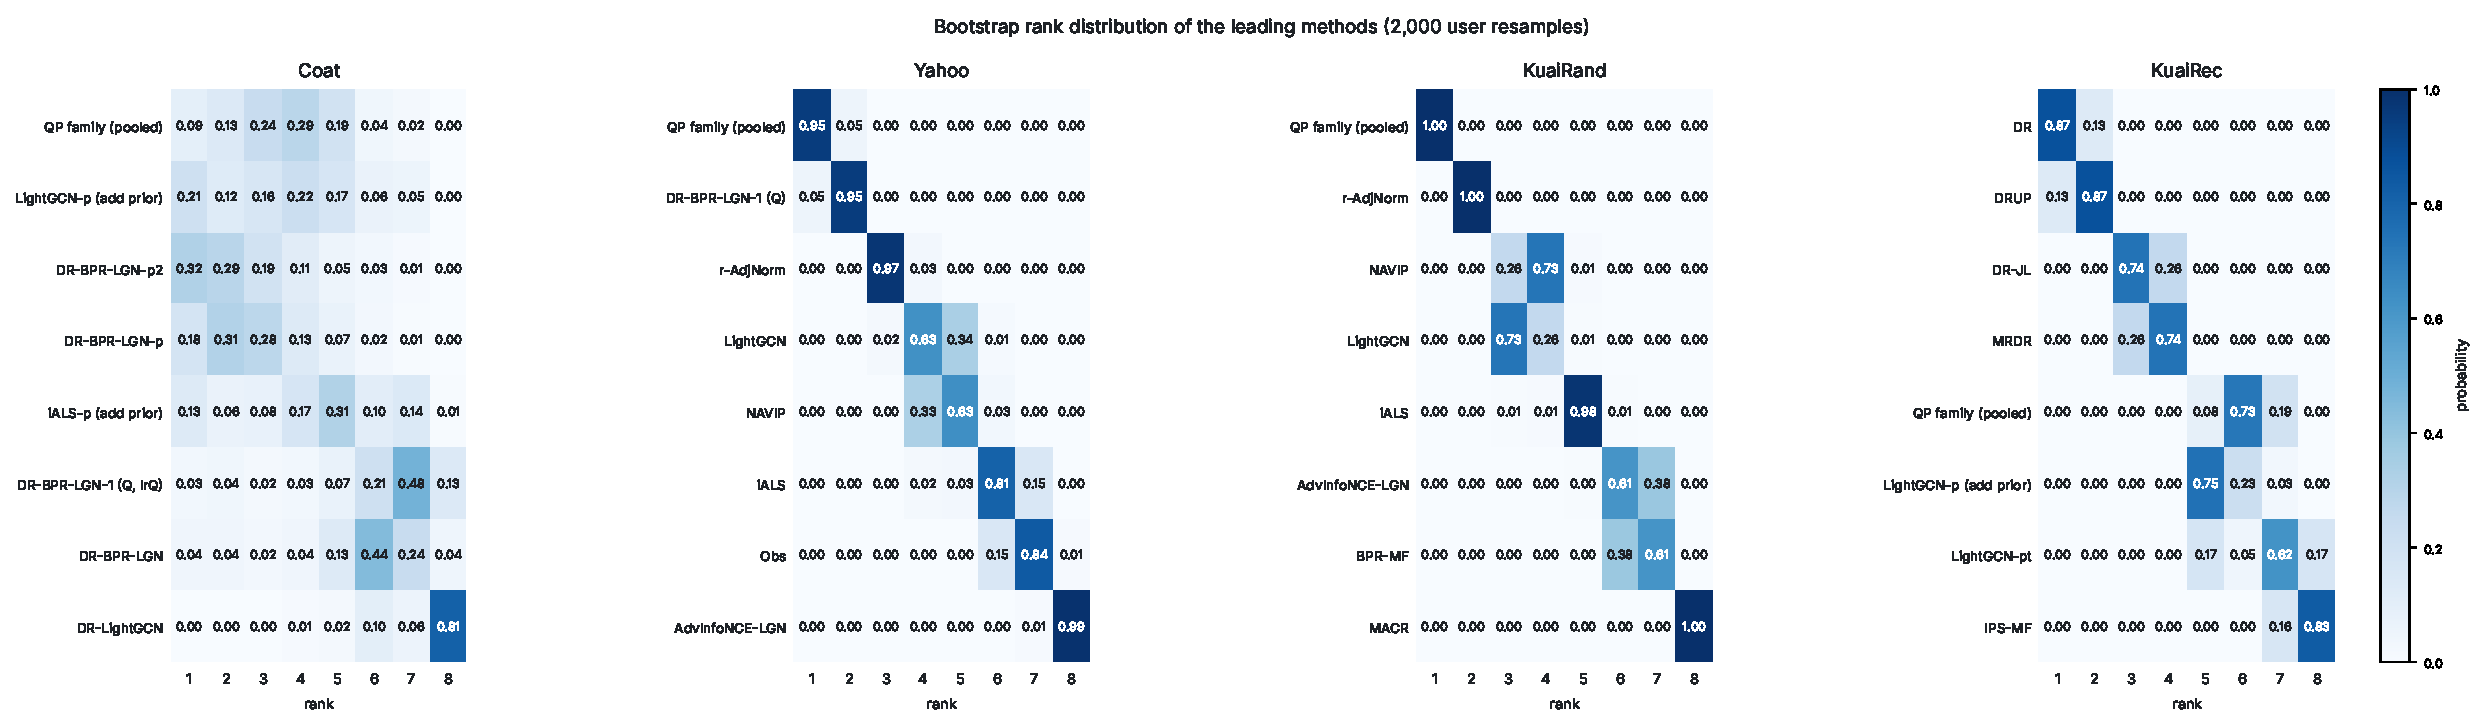
\includegraphics[width=\linewidth]{figs/rank_distribution}
\caption{Bootstrap rank distributions over 2,000 user resamples. For each dataset the rows are the eight methods with the highest mean validation score, excluding control rows, and the columns are the rank by mean test score (1 is best). On Coat the splits are resampled together with the users. Each cell gives the probability of that rank.}
\label{fig:rank}
\end{figure}

The bootstrap ranks (Figure~\ref{fig:rank}) show how stable the leader is. On Yahoo! R3 the QP family ranks first in 95.0\% of user resamples, and on KuaiRand in 99.8\%. On KuaiRec, DR and DRUP have the same mean score (0.6378) and exchange first place, with probabilities 0.873 and 0.127. The bootstrap therefore cannot separate them. On Coat no method is a stable leader. The most frequent first place is DR-BPR-LGN-p2, with probability 0.319, and the QP family ranks first with probability 0.090.

\subsection{What graph debiasing adds over an equally tuned backbone (RQ2)}\label{sec:res-debias}

On Coat the graph debiasers are not separated from LightGCN. The three with stored Coat results differ from it by $+3.76$ [5.74] (r-AdjNorm), $-1.59$ [10.13] (NAVIP) and $-0.65$ [30.16] (DR-LightGCN), and none of these is significant. Under the provisional margin of $\pm0.010$, the r-AdjNorm difference is equivalent to zero (TOST p = 0.017), while the NAVIP difference (p = 0.0515) and the DR-LightGCN difference (p = 0.271) are not. The minimum detectable difference for the primary comparison P1 on Coat is $43.07$ ($\times10^{-3}$), so the study cannot exclude a gain of that size for DR-LightGCN. On Coat, iALS differs from LightGCN by $+12.01$ [16.12] (p = 0.143, not significant).

On Yahoo! R3, r-AdjNorm is $+4.10$ [3.29] above LightGCN (p = 0.015, p$_\mathrm{Holm}$ = 0.029 in the two-comparison primary family). Adjusting over all comparisons with LightGCN in the appendix gives p$_\mathrm{Holm}$ = 0.073, and the Nadeau-Bengio correction for overlapping splits gives p$_\mathrm{Holm}$ = 0.883. On KuaiRand, r-AdjNorm is $+1.99$ [1.02] above LightGCN (p$_\mathrm{Holm}$ < 0.001). This difference lies inside the provisional margin of $\pm0.003$ (TOST p = 0.026), and the Nadeau-Bengio correction gives p$_\mathrm{Holm}$ = 1.000. Across Coat, Yahoo! R3 and KuaiRand, then, the best graph debiaser adds at most $+4.10$ ($\times10^{-3}$) nDCG over the equally tuned backbone, and the Nadeau-Bengio correction removes its significance.

KuaiRec, whose test matrix is fully observed, differs. DR-LightGCN is $+13.17$ [3.31] above LightGCN (p$_\mathrm{Holm}$ < 0.001) and NAVIP is $+10.41$ [1.82] above it (appendix). Under the Nadeau-Bengio correction the DR-LightGCN difference has p$_\mathrm{Holm}$ = 0.787. The pointwise LightGCN-pt, which has no debiasing, is $+19.59$ [4.55] above the BPR backbone. On KuaiRec, then, the change of loss contributes more than any graph debiaser does. The training-free operators are stronger still on this dataset (Section~\ref{sec:res-walk}).

The re-implementation of AdvInfoNCE is below LightGCN on all four datasets: $-46.47$ [25.16] on Coat, $-21.08$ [7.78] on Yahoo! R3, $-8.86$ [2.50] on KuaiRand and $-28.42$ [6.46] on KuaiRec, each significant under the appendix Holm adjustment. SimGCL and MACR are below LightGCN on all four datasets and significantly so on Yahoo! R3, KuaiRand and KuaiRec. On Coat, their differences ($-17.49$ [23.88] and $-29.43$ [24.60]) are not significant. These comparisons use our implementations, which are described in the protocol section.

Table~\ref{tab:T5} gives the primary comparisons with their Nadeau-Bengio columns. Under that correction, none of the four P1 comparisons is significant. The two P2 comparisons on KuaiRec remain significant, with p$_\mathrm{NB,Holm}$ of 0.009 for LightGCN-p and 0.043 for iALS-p. The P4 comparison, DRUP against DR-JL, is significant under the per-user test ($+4.38$ [2.21], p$_\mathrm{Holm}$ < 0.001) but not under the correction (p$_\mathrm{NB,Holm}$ = 0.426).

\begin{table}[t]
\centering
\footnotesize
\caption{Primary comparisons P1--P4 (Section 2.3): paired per-user differences, tests, MDE, TOST at the margins of Section 2.3, and the matched-budget difference at $k=k_\mathrm{min}$.}
\label{tab:T5}
\resizebox{\textwidth}{!}{%
\begin{tabular}{llllrrrrlrl}
\toprule
Dataset & Fam. & Comparison ($A-B$) & Diff.\ $\times10^{3}$ [95\% CI] & $p$ & $p_\mathrm{Holm}$ & $p_\mathrm{NB,Holm}$ & MDE $\times10^{3}$ & TOST at margin & Matched-$k$ diff $\times10^{3}$ & Seeds 1--3 diff $\times10^{3}$ \\
\midrule
Coat & P1 & DR-LightGCN -- LightGCN & -0.65 [30.16] & 0.966 & 1.000 & 1.000 & 43.07 & no ($p$=0.271) & +4.11 & -- \\
Coat & P2 & iALS-p (add prior) -- iALS & +16.82 [18.04] & 0.068 & 0.270 & 1.000 & 25.76 & no ($p$=0.771) & +16.12 & -- \\
Coat & P2 & LightGCN-p (add prior) -- LightGCN & +31.98 [20.65] & 0.003 & 0.013 & 1.000 & 29.48 & no ($p$=0.981) & +34.12 & -- \\
Coat & P3 & QP family (pooled) -- LightGCN-p (add prior) & +0.05 [8.29] & 0.991 & 1.000 & 1.000 & 11.83 & yes ($p$=0.009) & -0.36 & -- \\
Coat & P3 & DR-iALS -- iALS-p (add prior) & -10.22 [15.96] & 0.208 & 0.625 & 1.000 & 22.79 & no ($p$=0.511) & -11.21 & -- \\
Yahoo & P1 & r-AdjNorm -- LightGCN & +4.10 [3.29] & 0.015 & 0.029 & 0.883 & 4.70 & yes ($p$=0.000) & +2.87 & +5.26 ($p$=0.000) \\
Yahoo & P2 & LightGCN-p (add prior) -- LightGCN & -1.43 [3.93] & 0.475 & 0.475 & 0.883 & 5.62 & yes ($p$=0.000) & -2.16 & -- \\
KuaiRand & P1 & r-AdjNorm -- LightGCN & +1.99 [1.02] & 0.000 & 0.000 & 1.000 & 1.46 & yes ($p$=0.026) & +1.23 & +2.56 ($p$=0.000) \\
KuaiRand & P2 & LightGCN-p (add prior) -- LightGCN & -0.81 [1.33] & 0.234 & 0.234 & 1.000 & 1.90 & yes ($p$=0.001) & -0.79 & -- \\
KuaiRec & P1 & DR-LightGCN -- LightGCN & +13.17 [3.31] & 0.000 & 0.000 & 0.787 & 4.74 & no ($p$=1.000) & +12.97 & -- \\
KuaiRec & P2 & LightGCN-p (add prior) -- LightGCN & +21.22 [2.86] & 0.000 & 0.000 & 0.009 & 4.09 & no ($p$=1.000) & +20.25 & -- \\
KuaiRec & P2 & iALS-p (add prior) -- iALS & +14.74 [3.43] & 0.000 & 0.000 & 0.043 & 4.90 & no ($p$=1.000) & +16.89 & -- \\
KuaiRec & P3 & QP family (pooled) -- LightGCN-p (add prior) & -0.32 [0.50] & 0.211 & 0.211 & 0.871 & 0.72 & yes ($p$=0.000) & -0.12 & -- \\
KuaiRec & P4 & DRUP -- DR-JL & +4.38 [2.21] & 0.000 & 0.000 & 0.426 & 3.15 & no ($p$=0.890) & -14.90 & -- \\
\bottomrule
\end{tabular}}
\par\smallskip\raggedright\footnotesize Margins are the provisional values of Section 2.3 (TODO-L2 not yet closed). Seeds column: only comparisons whose baselines are in results/v4/seeds_*.json.
\end{table}


\subsection{Which ingredient carries the gain (RQ3)}\label{sec:res-ingredient}

The simple prior is the additive imputation $\hat\mu+b_u+b_i$, fitted once on the exposed log with inverse-propensity weights and added to the score as an offset. Within a user its ranking is the ranking of the item term $b_i$. Used as an offset on LightGCN (LightGCN-p), it gives $+31.98$ [20.65] on Coat (p$_\mathrm{Holm}$ = 0.013 in the primary family of Table~\ref{tab:T5}; 0.046 in the family of Table~\ref{tab:T9}), and $+21.22$ [2.86] on KuaiRec (p$_\mathrm{Holm}$ < 0.001). On Yahoo! R3 it gives $-1.43$ [3.93] (p$_\mathrm{Holm}$ = 0.475), and on KuaiRand $-0.81$ [1.33] (p$_\mathrm{Holm}$ = 0.234). The offset-only summary uses a different Holm family and reports 0.008 for Coat and 0.468 for KuaiRand. The offset helps on Coat and KuaiRec and not on Yahoo! R3 or KuaiRand. The tests here do not explain this pattern.

Table~\ref{tab:T9} separates the additive prior into its parts: the IPS weighting, the item term, and popularity. Removing the IPS weights does not reduce the gain. On KuaiRec, the unweighted prior added to iALS gives $+22.79$ [4.04] over iALS, and it exceeds the weighted prior by $+8.05$ [2.06] (p$_\mathrm{Holm}$ < 0.001). On Coat the unweighted prior is above the weighted one by $+6.27$ [6.97] for iALS and $+4.01$ [10.01] for LightGCN, neither significant. Popularity does not reproduce the effect on KuaiRec: its offset adds $+1.06$ [2.46] to iALS (p$_\mathrm{Holm}$ = 1.000), against $+14.74$ [3.43] for the weighted prior. Replacing the item term by a random permutation across items removes the KuaiRec gain and reverses it, with $-112.07$ [9.39] against iALS (p$_\mathrm{Holm}$ < 0.001). On Coat the same permutation gives $-14.06$ [18.53] for iALS and $-12.95$ [24.18] for LightGCN, neither significant, so the Coat result does not isolate the item term. The lowest offset weight of the grid was selected in all five KuaiRec splits for the shuffled item term, so the reported harm is an upper bound under that grid.

\begin{table}[t]
\centering
\footnotesize
\caption{Prior anatomy (X1). Test nDCG of iALS-p and LightGCN-p under four additive-imputation variants, and of the prior alone on all four datasets.}
\label{tab:T9}
\resizebox{\textwidth}{!}{%
\begin{tabular}{llrrrrr}
\toprule
Dataset & Learner / prior & nDCG (mean $\pm$ sd) & $\Delta$ vs no prior $\times10^{3}$ [CI] & $p_\mathrm{Holm}$ & $\Delta$ vs add $\times10^{3}$ [CI] & $p_\mathrm{Holm}$ \\
\midrule
Coat & iALS (no prior) & 0.5812 $\pm$ 0.0107 & -- & -- & -- & -- \\
Coat & iALS-p, add (IPS-fitted) & 0.5984 $\pm$ 0.0128 & +16.82 [18.04] & 0.811 & -- & -- \\
Coat & iALS-p, add, no IPS & 0.6044 $\pm$ 0.0115 & +23.08 [18.24] & 0.187 & +6.27 [6.97] & 0.856 \\
Coat & iALS-p, pop & 0.5832 $\pm$ 0.0238 & +1.67 [16.11] & 1.000 & -15.15 [15.39] & 0.698 \\
Coat & iALS-p, shuffled item bias & 0.5683 $\pm$ 0.0175 & -14.06 [18.53] & 1.000 & -30.87 [22.75] & 0.120 \\
Coat & LightGCN (no prior) & 0.5683 $\pm$ 0.0139 & -- & -- & -- & -- \\
Coat & LightGCN-p, add (IPS-fitted) & 0.6020 $\pm$ 0.0156 & +31.98 [20.65] & 0.046 & -- & -- \\
Coat & LightGCN-p, add, no IPS & 0.6052 $\pm$ 0.0145 & +36.00 [16.88] & $<$0.001 & +4.01 [10.01] & 1.000 \\
Coat & LightGCN-p, pop & 0.5835 $\pm$ 0.0233 & +15.63 [10.68] & 0.069 & -16.36 [19.52] & 1.000 \\
Coat & LightGCN-p, shuffled item bias & 0.5527 $\pm$ 0.0095 & -12.95 [24.18] & 1.000 & -44.93 [29.53] & 0.051 \\
KuaiRec & iALS (no prior) & 0.6133 $\pm$ 0.0030 & -- & -- & -- & -- \\
KuaiRec & iALS-p, add (IPS-fitted) & 0.6273 $\pm$ 0.0018 & +14.74 [3.43] & $<$0.001 & -- & -- \\
KuaiRec & iALS-p, add, no IPS & 0.6350 $\pm$ 0.0021 & +22.79 [4.04] & $<$0.001 & +8.05 [2.06] & $<$0.001 \\
KuaiRec & iALS-p, pop & 0.6144 $\pm$ 0.0028 & +1.06 [2.46] & 1.000 & -13.68 [3.31] & $<$0.001 \\
KuaiRec & iALS-p, shuffled item bias & 0.4993 $\pm$ 0.0032 & -112.07 [9.39] & $<$0.001 & -126.82 [9.29] & $<$0.001 \\
KuaiRec & LightGCN (no prior) & 0.6085 $\pm$ 0.0031 & -- & -- & -- & -- \\
KuaiRec & LightGCN-p, add (IPS-fitted) & 0.6288 $\pm$ 0.0023 & +21.22 [2.86] & $<$0.001 & -- & -- \\
Coat & prior alone, add (IPS-fitted) & 0.5585 $\pm$ 0.0105 & -- & -- & -- & -- \\
Coat & prior alone, add, no IPS & 0.5574 $\pm$ 0.0107 & -- & -- & -2.09 [8.46] & 1.000 \\
Coat & prior alone, pop & 0.5367 $\pm$ 0.0100 & -- & -- & -19.40 [27.79] & 1.000 \\
Coat & prior alone, shuffled item bias & 0.3572 $\pm$ 0.0125 & -- & -- & -203.62 [51.90] & $<$0.001 \\
Coat & prior alone, user only (b\_i = 0) & 0.3497 $\pm$ 0.0152 & -- & -- & -207.15 [49.91] & $<$0.001 \\
Yahoo & prior alone, add (IPS-fitted) & 0.5243 $\pm$ 0.0050 & -- & -- & -- & -- \\
Yahoo & prior alone, add, no IPS & 0.5237 $\pm$ 0.0055 & -- & -- & -1.09 [3.98] & 1.000 \\
Yahoo & prior alone, pop & 0.5331 $\pm$ 0.0065 & -- & -- & +8.90 [14.93] & 1.000 \\
Yahoo & prior alone, shuffled item bias & 0.3446 $\pm$ 0.0056 & -- & -- & -177.98 [17.37] & $<$0.001 \\
Yahoo & prior alone, user only (b\_i = 0) & 0.3767 $\pm$ 0.0051 & -- & -- & -144.74 [17.38] & $<$0.001 \\
KuaiRand & prior alone, add (IPS-fitted) & 0.3637 $\pm$ 0.0013 & -- & -- & -- & -- \\
KuaiRand & prior alone, add, no IPS & 0.3837 $\pm$ 0.0023 & -- & -- & +19.90 [2.45] & $<$0.001 \\
KuaiRand & prior alone, pop & 0.4204 $\pm$ 0.0021 & -- & -- & +56.41 [5.19] & $<$0.001 \\
KuaiRand & prior alone, shuffled item bias & 0.3257 $\pm$ 0.0018 & -- & -- & -39.12 [5.64] & $<$0.001 \\
KuaiRand & prior alone, user only (b\_i = 0) & 0.3259 $\pm$ 0.0011 & -- & -- & -38.84 [5.53] & $<$0.001 \\
KuaiRec & prior alone, add (IPS-fitted) & 0.6216 $\pm$ 0.0016 & -- & -- & -- & -- \\
KuaiRec & prior alone, add, no IPS & 0.6367 $\pm$ 0.0022 & -- & -- & +15.16 [1.68] & $<$0.001 \\
KuaiRec & prior alone, pop & 0.5766 $\pm$ 0.0026 & -- & -- & -45.70 [4.25] & $<$0.001 \\
KuaiRec & prior alone, shuffled item bias & 0.0398 $\pm$ 0.0007 & -- & -- & -582.01 [10.19] & $<$0.001 \\
KuaiRec & prior alone, user only (b\_i = 0) & 0.0686 $\pm$ 0.0010 & -- & -- & -554.01 [10.16] & $<$0.001 \\
\bottomrule
\end{tabular}}
\par\smallskip\raggedright\footnotesize $\Delta$ = per-user paired difference (mean over splits), $\times10^{3}$, [half-width of the 95\% CI]. No-prior references: stored iALS and LightGCN. The add row is the IPS-fitted additive prior. $p_\mathrm{Holm}$ over all paired tests of this table. user only (b\_i = 0) gives the same score to every item for a given user, so its ranking is decided by tie-breaking. Coat LightGCN-p and iALS-p use 10 splits, KuaiRec 5. Rows absent from the table were not run (only the prior-alone rows exist for those priors).
\end{table}


The training-free rows of Table~\ref{tab:T9} show the prior alone, with no learner. On KuaiRec the unweighted prior alone reaches $0.6367$, and the weighted prior alone $0.6216$. Popularity alone reaches $0.5766$. On KuaiRand the picture is different: popularity alone ($0.4204$) exceeds the weighted prior alone ($0.3637$) by $+56.41$ [5.19] (p$_\mathrm{Holm}$ < 0.001), and the unweighted prior alone ($0.3837$) exceeds the weighted one by $+19.90$ [2.45]. On Coat and Yahoo! R3, popularity alone is not significantly different from the weighted prior alone. The paired tests in the table are between the variants of the prior. No paired test of the prior alone against the training-free DRUP operator is in the result files, so the $0.0011$ gap between the unweighted prior alone and DRUP on KuaiRec is reported as a difference of means only.

The weights on the sampled negatives form the second ingredient. On Yahoo! R3 the weights without the offset (DR-BPR-LGN-1) exceed LightGCN-p by $+15.15$ [5.84] (p$_\mathrm{Holm}$ < 0.001), and the QP family exceeds LightGCN-p on KuaiRand by $+4.74$ [1.54] (p$_\mathrm{Holm}$ < 0.001). A shuffled Q removes the Yahoo! R3 gain, with $-1.01$ [3.20] against LightGCN (p$_\mathrm{Holm}$ = 0.534). On Coat, shuffled Q gives $+0.97$ [5.50] against LightGCN (p$_\mathrm{Holm}$ = 0.73), while popularity weights give $+6.91$ [6.04] (p$_\mathrm{Holm}$ = 0.0505, not significant). On Yahoo! R3, popularity weights are significantly below LightGCN ($-15.91$ [6.06], p$_\mathrm{Holm}$ < 0.001). On KuaiRand the validated combination selected $\beta=0$ in four of five splits, so the gain there comes from the weights.

The refinements built on the prior do not improve on it where the prior is tested. On Coat, the QP family is equivalent to LightGCN-p within $\pm0.010$ ($+0.05$ [8.29], TOST p = 0.009). The largest refinement difference from LightGCN-p is $+3.27$ [6.94] (DR-BPR-LGN-p2), which is not significant. The Q-only variants are $-8.02$ [18.85] and $-10.79$ [19.26] below it. On iALS, DR-iALS is $-10.22$ [15.96] against iALS-p (p$_\mathrm{Holm}$ = 0.208). On KuaiRec the QP family is $-0.32$ [0.50] against LightGCN-p (p$_\mathrm{Holm}$ = 0.211, equivalent within $\pm0.003$). Every refinement in the study is below DRUP ($0.6378$) on KuaiRec. The DRGP refinement, which uses a leave-edge-out DR-fitted prior, reaches $0.6318$, which is $-5.58$ [1.90] against DRUP (p$_\mathrm{Holm}$ < 0.0001). These DRGP results are stage-1 results without seeds, and DRGP was run on Coat and KuaiRec only. Its Coat score of $0.5992$ is $-0.13$ [15.11] against \qp{} (p$_\mathrm{Holm}$ = 1.000). A validated ensemble of \qp{} and DRUP selects one component in most splits and does not add to either: DRUP in four of five KuaiRec splits and \qp{} in nine of ten Coat splits. On KuaiRec the ensemble is $-0.18$ [0.19] against DRUP (p$_\mathrm{Holm}$ = 0.0664), and on Coat it is $+1.79$ [2.39] against \qp{} (p$_\mathrm{Holm}$ = 0.1421).

\begin{table}[t]
\centering
\footnotesize
\caption{Refinement family against the simple debiased prior of the same learner, and the shuffled and popularity controls against the backbone.}
\label{tab:T6}
\resizebox{\textwidth}{!}{%
\begin{tabular}{lllrrlrrl}
\toprule
Dataset & Family & Method & Mean & Cfg & Versus & Diff.\ $\times10^{3}$ [95\% CI] & $p_\mathrm{Holm}$ & TOST (Coat: exclusion, not equivalence) \\
\midrule
Coat & refinement vs simple prior & DR-BPR-LGN & 0.5912 & 108 & LightGCN-p (add prior) & -8.02 [18.85] & 1.000 & does not exclude \\
Coat & refinement vs simple prior & DR-BPR-LGN-1 (Q-only) & 0.5887 & 54 & LightGCN-p (add prior) & -10.79 [19.26] & 1.000 & does not exclude \\
Coat & refinement vs simple prior & DR-BPR-LGN-p & 0.6039 & 108 & LightGCN-p (add prior) & +2.09 [6.48] & 1.000 & excludes $\lvert d\rvert>0.010$ \\
Coat & refinement vs simple prior & DR-BPR-LGN-p2 & 0.6046 & 108 & LightGCN-p (add prior) & +3.27 [6.94] & 1.000 & excludes $\lvert d\rvert>0.010$ \\
Coat & refinement vs simple prior & QP family (pooled) & 0.6015 & 324 & LightGCN-p (add prior) & +0.05 [8.29] & 1.000 & excludes $\lvert d\rvert>0.010$ \\
Coat & refinement vs simple prior (iALS) & DR-iALS & 0.5871 & 48 & iALS-p (add prior) & -10.22 [15.96] & 0.208 & does not exclude \\
Coat & controls vs backbone & control: shuffled Q & 0.5689 & 54 & LightGCN & +0.97 [5.50] & 0.730 & excludes $\lvert d\rvert>0.010$ \\
Coat & controls vs backbone & control: popularity Q & 0.5751 & 54 & LightGCN & +6.91 [6.04] & 0.050 & does not exclude \\
Yahoo & refinement vs simple prior & DR-BPR-LGN-1 (Q-only) & 0.6837 & 36 & LightGCN-p (add prior) & +15.15 [5.84] & $<$0.001 & no \\
Yahoo & refinement vs simple prior & QP family (pooled) & 0.6866 & 84 & LightGCN-p (add prior) & +18.20 [5.64] & $<$0.001 & no \\
Yahoo & controls vs backbone & control: shuffled Q & 0.6689 & 12 & LightGCN & -1.01 [3.20] & 0.534 & yes \\
Yahoo & controls vs backbone & control: popularity Q & 0.6550 & 12 & LightGCN & -15.91 [6.06] & $<$0.001 & no \\
KuaiRand & refinement vs simple prior & QP family (pooled) & 0.4613 & 30 & LightGCN-p (add prior) & +4.74 [1.54] & $<$0.001 & no \\
KuaiRec & refinement vs simple prior & QP family (pooled) & 0.6285 & 120 & LightGCN-p (add prior) & -0.32 [0.50] & 0.211 & yes \\
\bottomrule
\end{tabular}}
\par\smallskip\raggedright\footnotesize Holm within each family and dataset. Rows are missing where the simple prior has not been run for that dataset.
\end{table}


Two checks on the prior concern its inputs. The first is the propensity model. Coat's shipped propensities were estimated by the dataset authors from the uniform sample, so we refitted them with the estimator used on the other three datasets. Table~\ref{tab:T10} shows that this changes little. The estimated-minus-shipped difference is $+2.63$ [5.27] for iALS-p and $+1.64$ [10.30] for LightGCN-p, and the imputation alone changes by $-1.14$ [7.26]. None is significant. The gain over the no-prior reference remains: $+19.44$ [18.66] for iALS-p and $+33.62$ [16.72] for LightGCN-p. The estimated-propensity run of LightGCN was not carried out.

\begin{table}[t]
\centering
\footnotesize
\caption{Coat with estimated propensities (X2): --prop pop versus the shipped propensities.}
\label{tab:T10}
\resizebox{\textwidth}{!}{%
\begin{tabular}{llrrrrr}
\toprule
Method & Propensities & nDCG (mean $\pm$ sd) & $\Delta$ vs no-prior $\times10^{3}$ [CI] & $p_\mathrm{Holm}$ & Estimated $-$ shipped $\times10^{3}$ [CI] & $p_\mathrm{Holm}$ \\
\midrule
iALS-p & shipped & 0.5984 $\pm$ 0.0128 & +16.82 [18.04] & 0.380 & -- & -- \\
iALS-p & estimated & 0.6009 $\pm$ 0.0120 & +19.44 [18.66] & 0.330 & +2.63 [5.27] & 1.000 \\
LightGCN-p & shipped & 0.6020 $\pm$ 0.0156 & +31.98 [20.65] & 0.023 & -- & -- \\
LightGCN-p & estimated & 0.6025 $\pm$ 0.0154 & +33.62 [16.72] & $<$0.001 & +1.64 [10.30] & 1.000 \\
iALS-wide & shipped & 0.5869 $\pm$ 0.0124 & +7.39 [7.52] & 0.380 & -- & -- \\
iALS-wide & estimated & 0.5869 $\pm$ 0.0124 & +7.39 [7.52] & 0.380 & 0 (identical) & 1 \\
imputation alone (add) & shipped & 0.5585 $\pm$ 0.0105 & -- & -- & -- & -- \\
imputation alone (add) & estimated & 0.5573 $\pm$ 0.0097 & -- & -- & -1.14 [7.26] & 1.000 \\
iALS (no prior) & shipped & 0.5812 $\pm$ 0.0107 & -- & -- & -- & -- \\
LightGCN (no prior) & shipped & 0.5683 $\pm$ 0.0139 & -- & -- & -- & -- \\
\bottomrule
\end{tabular}}
\par\smallskip\raggedright\footnotesize The no-prior reference of each learner is the stored run. Plain iALS and LightGCN do not read the propensities (only NAVIP does), so the shipped no-prior run is the reference for the estimated rows. LightGCN with estimated propensities was not run. $p_\mathrm{Holm}$ over the tests of this table.
\end{table}


The second check is the tuning budget of the backbone. The stored iALS grid selects its largest value of the confidence weight $\alpha$ (30) in all 10 splits, and the wider grid of Table~\ref{tab:T11} selects its largest value (1000) in four splits. The stored grid is therefore bounded at its edge, and the wider grid is not exhausted. Over the stored iALS, the wider grid gives $+12.92$ [8.01] (p$_\mathrm{Holm}$ = 0.003), against $+16.82$ [18.04] for the offset model over the same stored iALS. The wider grid is not significantly different from iALS-p ($-3.90$ [15.99], p$_\mathrm{Holm}$ = 0.631). In this comparison, most of the Coat gap between iALS and the prior-augmented model is a matter of tuning budget, and the wider grid is still not exhausted.

\begin{table}[t]
\centering
\footnotesize
\caption{Coat iALS with the wider grid (X4) against the stored iALS and iALS-p.}
\label{tab:T11}
\resizebox{\textwidth}{!}{%
\begin{tabular}{llrrrrrrl}
\toprule
Model & Grid & Cfg & nDCG (mean $\pm$ sd) & $\Delta$ vs iALS $\times10^{3}$ [CI] & $p_\mathrm{Holm}$ & $\Delta$ vs iALS-p $\times10^{3}$ [CI] & $p_\mathrm{Holm}$ & Selected values (number of splits) \\
\midrule
iALS (stored) & alpha \{3,10,30\} x reg \{1,10,100,1000\} x dim \{32,64\} & 24 & 0.5812 $\pm$ 0.0107 & ref. & -- & -- & -- & alpha 30:10; reg 100:10 \\
iALS-wide (v5 grid) & alpha \{10,30,100\} x reg \{10,100,300\} x dim \{32,64\} & 18 & 0.5869 $\pm$ 0.0124 & -- & -- & -- & -- & alpha 30:1, 100:9; reg 100:4, 300:6 \\
iALS-wide2 (X4 grid) & alpha \{30,100,300,1000\} x reg \{10,100,300,1000\} x dim \{32,64\} & 32 & 0.5922 $\pm$ 0.0150 & +12.92 [8.01] & 0.003 & -3.90 [15.99] & 0.631 & alpha 30:1, 100:4, 300:1, 1000:4; reg 100:2, 300:3, 1000:5 \\
iALS-p add (stored) & alpha \{10,30,100\} x reg \{10,100,300\} x pbeta \{0.1,0.2,0.3,0.5,1\} x dim \{32,64\} & 90 & 0.5984 $\pm$ 0.0128 & -- & -- & -- & -- & alpha 30:2, 100:8; reg 100:4, 300:6 \\
\bottomrule
\end{tabular}}
\par\smallskip\raggedright\footnotesize $\Delta$ = per-user paired difference (mean over the 10 splits), $\times10^{3}$, [half-width of the 95\% CI]. $p_\mathrm{Holm}$ over the two comparisons of iALS-wide2. Selected values are counted over the 10 splits.
\end{table}


\subsection{Exact unbiasedness of the propagation and the training-free results (RQ4)}\label{sec:res-walk}

The walk correction removes the repeated-edge terms of multi-hop doubly robust propagation. On a synthetic MNAR model, it reduces the relative $|\mathrm{bias}|$ of the DR adjacency from $1.756$ to $0.019$ at $K=3$ and from $8.350$ to $0.039$ at $K=5$. On a semi-synthetic KuaiRec log with true propensities and fixed degree weights, DRUP minus DR nDCG@20 is positive at $\beta\in\{0.3,1,3\}$ in all six cells, between $+12.5$ and $+19.6$ ($\times10^{-3}$) at $\beta=0.3$. It reverses at $\beta=1000$ in two cells, reaching $-5.35$ ($\times10^{-3}$). In the imputation-degree cell of the same study, DR reaches $0.377$ and DRUP $0.370$. The gain therefore appears with known propensities and fixed degree weights, and it does not appear in the one cell we ran with estimated degree weights.

On the real logs the correction does not help at matched configurations. On Coat, DRUP minus DR is negative at every value of $\beta$ in the grid, from $-0.33$ at $\beta=0.03$ to $-8.17$ at $\beta=1000$, and it is negative in all ten splits for $\beta\geq0.3$. On Yahoo! R3 the differences are small and negative, from $-0.02$ to $-0.32$. Among the selected runs, the difference is $+1.40$ [3.86] on Coat (p$_\mathrm{Holm}$ = 0.475), within the margin of $\pm0.010$ (TOST p < 0.001). On KuaiRec the selected-run difference is $-0.12$ [0.15] (p$_\mathrm{Holm}$ = 0.113), within $\pm0.003$ (TOST p < 0.001). Table~\ref{tab:T8} gives the matched-configuration and selected-run values.

\begin{table}[htbp]
\centering
\footnotesize
\caption{Walk correction (DRUP minus DR) at matched configurations and in the selected runs.}
\label{tab:T8}
\resizebox{\textwidth}{!}{%
\begin{tabular}{lllrrr}
\toprule
Dataset & $\beta$ & Mean diff.\ $\times10^{3}$ [95\% CI] & Share of configs $<0$ & Splits with mean $<0$ & $p_\mathrm{Holm}$ \\
\midrule
\multicolumn{6}{l}{\emph{Matched configurations (split means, no test)}} \\
Coat & 0.03 & -0.33 & 0.49 & 7/10 & -- \\
Coat & 0.1 & -1.28 & 0.52 & 9/10 & -- \\
Coat & 0.3 & -2.92 & 0.54 & 10/10 & -- \\
Coat & 1 & -5.09 & 0.74 & 10/10 & -- \\
Coat & 3 & -7.35 & 0.74 & 10/10 & -- \\
Coat & 10 & -7.44 & 0.80 & 10/10 & -- \\
Coat & 1000 & -8.17 & 0.90 & 10/10 & -- \\
Yahoo & 0.03 & -0.02 & 0.41 & 5/5 & -- \\
Yahoo & 0.1 & -0.03 & 0.50 & 4/5 & -- \\
Yahoo & 0.3 & -0.12 & 0.56 & 5/5 & -- \\
Yahoo & 1 & -0.04 & 0.47 & 3/5 & -- \\
Yahoo & 3 & -0.07 & 0.28 & 4/5 & -- \\
Yahoo & 10 & -0.19 & 0.41 & 5/5 & -- \\
Yahoo & 1000 & -0.32 & 0.38 & 5/5 & -- \\
\multicolumn{6}{l}{\emph{Selected runs (per-user paired test)}} \\
Coat & -- & +1.40 [3.86] & -- & -- & 0.475 \\
Yahoo & -- & +0.00 [0.00] & -- & -- & 1.000 \\
KuaiRec & -- & -0.12 [0.15] & -- & -- & 0.113 \\
\bottomrule
\end{tabular}}
\par\smallskip\raggedright\footnotesize Panel A: difference of the matched-configuration split means, $\times10^{3}$; the last column is the number of splits with a negative mean. Panel B: per-user differences with 95\% half-widths in brackets, and Holm-adjusted $p$ within the walk family. Coat: differences larger than $\pm$0.010 are excluded (TOST $p<0.001$); equivalence is not claimed. On Yahoo! R3 the selected DRUP and DR runs give identical per-user values, so the walk correction changes nothing there and the row is uninformative. KuaiRec: TOST within the sensitivity margin ($\pm$0.003), $p<0.001$.
\end{table}


Among the training-free operators, the KuaiRec result goes to doubly robust propagation, not to the walk correction. DRUP reaches $0.6378$ and the DR adjacency on which it is built also reaches $0.6378$, and a five-hop DR adjacency reaches $0.6379$. No trained model in Table~\ref{tab:T4} exceeds $0.6378$ on KuaiRec: the best is DR-JL at $0.6332$, and the QP family reaches $0.6285$. On Coat, DRUP is weak at $0.5467$, and on Yahoo! R3 the DRUP and DR rows coincide at $0.6567$. In the bootstrap, DR ranks first in 87.3\% of resamples on KuaiRec and DRUP in 12.7\% (Figure~\ref{fig:rank}), which reflects the tie in their means. The unweighted prior alone ($0.6367$) is the one training-free result close to DRUP, and it is reported in Table~\ref{tab:T9}. Table~\ref{tab:T4} gives the imputation row on KuaiRec as $0.6194$, against $0.6216$ for the prior alone in Table~\ref{tab:T9}. These come from separate fits, and the stored results do not record why they differ.

\section{Discussion}\label{sec:discussion}

\subsection{What the evidence supports}\label{sec:disc-support}

Under a protocol that keeps uniform data out of training, apart from Coat's shipped propensities, and selects on validation data, the ranking of debiasing methods depends on evaluation choices in ways that matter at the scale of the differences being compared. Selecting on test data inflates the Coat scores by up to $0.030$ nDCG@5 and reverses the order of iALS and LightGCN. The differences among the leading Coat methods are of the same order (Table~\ref{tab:T4}), so a ranking of those methods made on test data is not reliable without the validation step.

Graph-specific debiasing adds little over an equally tuned backbone on Coat, Yahoo! R3 and KuaiRand. The largest gain over LightGCN on these three datasets is $+4.10$ ($\times10^{-3}$) nDCG, for r-AdjNorm on Yahoo! R3, and the Nadeau-Bengio correction removes its significance. KuaiRec is different. NAVIP and DR-LightGCN add $+10.41$ and $+13.17$ ($\times10^{-3}$) there, although r-AdjNorm adds only $+0.22$, and a change of training loss without any debiasing adds $+19.59$. A reader comparing debiasers on KuaiRec therefore needs the pointwise backbone as the reference, not only the BPR one.

On Coat and KuaiRec the additive prior is the ingredient with the largest effect that we tested. Added as a score offset to LightGCN, it gives $+31.98$ [20.65] on Coat and $+21.22$ [2.86] on KuaiRec, and it does not change Yahoo! R3 or KuaiRand. The evidence does not show that the inverse-propensity weighting matters: on KuaiRec the unweighted prior is significantly better than the weighted one, and on Coat it is numerically higher without a significant difference. A random permutation of the item term removes the KuaiRec gain, but on Coat the same permutation does not significantly change the score, so the item term is established on KuaiRec and not on Coat. These results do not establish why the prior helps. The reading that the item term uses exposed negatives that a BPR objective discards is a hypothesis, and the prior-alone comparisons do not test it.

On Yahoo! R3 and KuaiRand the weights on the sampled negatives carry the gain. On Yahoo! R3 a shuffled weight vector removes it; no shuffled control was run on KuaiRand. Popularity weights are significantly below LightGCN on Yahoo! R3, so the weights are not a popularity reweighting. On KuaiRand, however, the popularity prior alone outperforms the IPS-fitted prior alone by $+56.41$ [5.19], so the simple non-personalised baseline is a serious competitor there, and a study that omits it would overstate the debiased prior.

On KuaiRec, training-free doubly robust propagation has the highest mean in Table~\ref{tab:T4}, and no trained method or refinement in the study exceeds it. The walk correction that makes its propagation exactly unbiased on synthetic logs does not change accuracy on the real logs at matched configurations. For ranking, then, the bias that the correction removes is not the limiting factor in these data.

Finally, the backbone matters as much as the debiaser. A wider iALS grid on Coat raises the stored iALS by $+12.92$ [8.01] (p$_\mathrm{Holm}$ = 0.003), against $+16.82$ [18.04] for the offset model over the same stored iALS. An evaluation that tunes the proposed method more than its baselines can produce a gap of that size from budget alone.

\subsection{Implications for evaluating debiasing methods}\label{sec:disc-implications}

The results support the following practices. Each item rests on a result above.

\begin{enumerate}
\item \textbf{Keep uniform data out of training, and state where every nuisance comes from.} Coat's shipped propensities came from the uniform sample. Refitting them with the estimator used on the other datasets changes the Coat prior results by at most $+2.63$ [5.27] (Table~\ref{tab:T10}). The check is cheap, and it should be reported whenever the propensities are not fitted on the training log.
\item \textbf{Select per split on validation data, and report the test-oracle gap.} The gap is $+0.0097$ to $+0.0302$ on Coat, and it reverses the order of iALS and LightGCN there (Section~\ref{sec:res-eval}).
\item \textbf{Report the budget, and compare at matched budget.} Grid sizes in these experiments range from 6 to 324 configurations. The sign of the DRUP comparison with DR-JL on KuaiRec changes in 78.4\% of six-configuration subgrids (Table~\ref{tab:T7}).
\item \textbf{Include the simple baselines as mandatory rows:} the IPS imputation alone, a tuned iALS with its wider grid, pointwise LightGCN, the popularity ranker, and the backbone with the debiased prior. Several of these changed a conclusion here: pointwise LightGCN on KuaiRec ($+19.59$ [4.55] over the BPR backbone), popularity against the prior alone on KuaiRand, and the wider iALS grid on Coat.
\item \textbf{Retrain the selected configurations with several seeds.} On Coat, the difference between \qp{} and iALS is $+20.02$ [19.74] (p$_\mathrm{Holm}$ = 0.0469) in the main run and $+3.39$ [20.70] (p$_\mathrm{Holm}$ = 0.747) over seeds 1 to 3.
\item \textbf{Report the minimum detectable difference with every claim of no difference, and test equivalence with a margin fixed in advance.} On Coat the minimum detectable difference for the primary comparisons is $0.012$ to $0.043$, which is large relative to the method differences in Table~\ref{tab:T4}.
\item \textbf{Use a correction for overlapping splits, and report it next to the standard test.} Under the Nadeau-Bengio correction, no graph-debiaser comparison (P1) is significant on any dataset.
\item \textbf{Publish the per-split validation and test results.} The selection analyses here, including the inflation, the subgrid stability and the bootstrap ranks, can be redone only from per-split values.
\end{enumerate}

\subsection{Limitations and threats to validity}\label{sec:disc-limits}

\begin{enumerate}
\item \textbf{Power on Coat.} Coat has 225 evaluated users. The minimum detectable differences of the primary comparisons range from $0.012$ to $0.043$. Coat results are therefore statements of the form ``no detectable difference, and differences larger than the stated margin are excluded'', never statements of equivalence.
\item \textbf{Provisional equivalence margins.} The TOST margins ($\pm0.010$ on Coat and Yahoo! R3, $\pm0.003$ on KuaiRand and KuaiRec) were declared before the analysis. They have not yet been checked against published effect sizes, and they should be read as provisional.
\item \textbf{Our implementations.} The graph baselines NAVIP, r-AdjNorm, SimGCL and MACR, and the refinements, are our implementations. AdvInfoNCE is a simplified re-implementation: its adversary budget is implicit, it has no KL-ball projection, and its grid differs across datasets. The official AdvInfoNCE code and the PPD post-hoc method were not run. The negative results for these methods are therefore about our implementations under this protocol.
\item \textbf{The refinement family is ours.} The seven refinements (Section~\ref{sec:res-ingredient}) were developed as candidate methods before this study, and they are reported in full with their configuration counts. The family is not exhaustive, and the results do not show that no other refinement helps.
\item \textbf{Seeds are incomplete.} Seeds 1 to 3 were not run for the Coat prior rows. Seed checks cover the leading methods only. DRGP was run on Coat and KuaiRec only, and its KuaiRec and Coat stage-1 results have no seeds.
\item \textbf{Budgets are unequal and only partly matched.} Matched-budget differences are split means without tests. The sensitivity analysis draws random subgrids of the stored configurations, not new searches.
\item \textbf{Grid edges.} On KuaiRec, the popularity and shuffled priors select the lowest offset weight of their grid in all five splits, so the reported shuffled-prior harm is an upper bound under that grid. On KuaiRec the unweighted prior selects the largest regularisation value of its grid (1000). The wider iALS grid is not exhausted.
\item \textbf{Incomplete ablations.} The user-only prior was run only as a prior alone and not in a learner. LightGCN with estimated propensities was not run. On KuaiRec, only the additive prior was run in the offset-only LightGCN setting.
\item \textbf{Replay gaps.} Replaying each stored selection from its bank reproduces 151 of 154 method means within 0.002. Three do not. On replay the KuaiRec DR-LightGCN mean is $0.0033$ higher than the stored $0.6212$, the Yahoo! R3 DR-LightGCN mean $0.0058$ higher, and the Yahoo! R3 MACR mean $0.0060$ higher. The stored values are reproduced only with an early-stopping setting that the bank does not record. The KuaiRec and Yahoo! R3 DR-LightGCN values appear in Table~\ref{tab:T4}, and the KuaiRec value also enters the P1 comparison of Table~\ref{tab:T5}.
\item \textbf{Family dependence.} Several p-values change with the Holm family. The Yahoo! R3 r-AdjNorm comparison has p$_\mathrm{Holm}$ = 0.029 in the primary family and 0.073 over all comparisons with LightGCN. The Coat offset comparison has 0.013 in the primary family and 0.046 in the family of the prior-anatomy table. We report the family with each value.
\item \textbf{Overlapping splits.} Per-user tests over overlapping splits treat the log and the fitted nuisances as fixed, and they can be anti-conservative. The Nadeau-Bengio correction removes significance from every P1 comparison.
\item \textbf{Exposure semantics.} On Coat and Yahoo! R3, exposure is user self-selection. The derivation of the weights assumes that exposure is independent of the outcome given the covariates of the propensity model.
\item \textbf{Test design.} We report one K per dataset in the main text (nDCG@5 on Coat and Yahoo! R3, nDCG@10 on KuaiRand, nDCG@20 on KuaiRec). The alternative metric is computed on the stored selections only. KuaiRec has a fully observed test matrix with about 3,300 candidates per user, which differs from the other three datasets, and we have no test of which feature causes the difference.
\item \textbf{Unexplained differences.} Two fits of the imputation prior on KuaiRec give $0.6194$ and $0.6216$ (Table~\ref{tab:T4} and Table~\ref{tab:T9}). No paired test compares the prior alone with DRUP, so the $0.0011$ gap to DRUP is a difference of means.
\item \textbf{Synthetic evidence for the walk correction.} The bias results come from a synthetic MNAR model and a semi-synthetic KuaiRec study. Their gains do not carry over to the real logs at matched configurations.
\item \textbf{The mechanism is untested.} The item-term reading in Section~\ref{sec:disc-support} is a hypothesis. The results show that an item-level term fitted once on the exposed log carries the effect on KuaiRec. They do not show why.
\end{enumerate}

\section{Conclusion}\label{sec:conclusion}

We re-evaluated exposure-bias corrections for graph recommenders on four benchmarks with uniformly exposed test data,
under one protocol in which uniform data serve for validation and testing, and, through Coat's shipped propensities,
for one nuisance that we check for the prior rows. The study asked how much evaluation choices move conclusions, how
much graph-specific debiasing adds over an equally tuned backbone, which ingredient carries the gains that remain, and
whether exact unbiasedness of the propagation matters for ranking.

First, the protocol is sensitive to evaluation choices. Selecting on test data inflates Coat scores by up to $0.030$
nDCG@5, and under the per-split test oracle it reverses the order of iALS and LightGCN. The search space of a backbone
can move a baseline by an amount comparable to the gain of a prior. Second, third-party graph-specific debiasers add at
most $+4.10\times10^{-3}$ nDCG over LightGCN in the point estimates on Coat, Yahoo! R3 and KuaiRand-Pure, and none of
these gains survives the correction for overlapping splits on those datasets. On KuaiRec the gains are larger, NAVIP's
gain survives the correction, and a pointwise loss without any debiasing gives a larger mean difference. The QP-LightGCN
family is not significant under the correction on Yahoo! R3 or KuaiRand-Pure. Third, an additive prior, fitted once on
the exposed log and added to the score, gives the largest point-estimate gains over LightGCN on Coat and KuaiRec. The
Coat gain is not robust to the correction for overlapping splits, and the KuaiRec gain is. Removing the
inverse-propensity weights does not reduce the gain, a shuffled item term removes the KuaiRec gain, and popularity does
not reproduce it. The mechanism is not identified. Fourth, the walk correction, which makes multi-hop doubly robust
propagation exactly unbiased, does not improve ranking on Coat, Yahoo! R3 or KuaiRec. In a semi-synthetic KuaiRec study
with known labels, DRUP has the higher nDCG@20 in seven of nine cells. That setting differs from the real logs, and we
do not take it to show that the correction helps there. DR and DRUP were not run on KuaiRand-Pure.

The study does not propose a method. It does not show that debiasing is ineffective in general, because its scope is
four public benchmarks, one cut-off per dataset and offline evaluation of implicit-feedback learners trained on the
biased log. It does not establish equivalence on Coat, where the study is underpowered. For evaluation, the practical
requirements are to select per split on validation data, to match budgets, to include the simple baselines, and to
report minimum detectable effects and corrected tests with every claim that two methods are equal or that one is
better.

\bibliographystyle{elsarticle-harv}
\bibliography{../refs,refs_new}
\end{document}
